% This is samplepaper.tex, a sample chapter demonstrating the
% LLNCS macro package for Springer Computer Science proceedings;
% Version 2.20 of 2017/10/04
%
\documentclass[runningheads]{llncs}
%
\usepackage{graphicx}
\usepackage{algpseudocode}
\usepackage{amsmath, amssymb, enumitem}
\usepackage[table,xcdraw]{xcolor}
\usepackage{dblfloatfix}
\usepackage{subfig}
\usepackage[colorinlistoftodos]{todonotes}
\setuptodonotes{inline}
% Used for displaying a sample figure. If possible, figure files should
% be included in EPS format.
%
% If you use the hyperref package, please uncomment the following line
% to display URLs in blue roman font according to Springer's eBook style:
% \renewcommand\UrlFont{\color{blue}\rmfamily}

\begin{document}
%
\title{Mining Invariants from State Space Observations\thanks{Supported by EPSRC and Siemens Mobility UK}}
%
%\titlerunning{Abbreviated paper title}
% If the paper title is too long for the running head, you can set
% an abbreviated paper title here
%
\author{Ben Lloyd-Roberts\inst{1} \and
Michael Edwards\inst{1} \and {Phillip James}\inst{1}}
%
\authorrunning{Lloyd-Roberts et al.}
% First names are abbreviated in the running head.
% If there are more than two authors, 'et al.' is used.
%
\institute{Swansea University, United Kingdom \\
\email{\{ben.lloyd-roberts, michael.edwards, p.d.james\}@swansea.ac.uk}}
%
\maketitle              % typeset the header of the contribution
%
\begin{abstract}
The application of formal methods to verify that railway signalling systems operate correctly is well established within academia and is beginning to see real applications. However, there is yet to be a substantial impact within industry due to current approaches often producing false positive results that require lengthy manual analysis. It is accepted that invariants, properties which hold for all states under which a signalling system operates, can help reduce occurrences of false positives. However automated deduction of these invariant remains a challenge. In this work we report on using reinforcement learning to explore state spaces of signalling systems and generate a dataset of state spaces from which we envisage invariants could be mined. Our results suggest the viability of reinforcement learning in both maximising state space coverage and estimating the longest loop free path for state spaces. Additionally, we use experiences observed by our agents to compute the phi coefficient between sets of variables across unique states. This allows us to both infer invariant properties across states and inform agent exploration by converging coefficients over time.

\keywords{First keyword  \and Second keyword \and Another keyword.}
\end{abstract}
%
%
%
\section{Introduction}\todo{Review / reframe for invariant approach}
Model checking is a formal verification technique stemming from the need to systematically
check whether certain properties hold for different configurations (states) of a given system.
Given a transition system $T$ and a formula (or property) $F$, model checking attempts to verify through refutation that $s \vdash F$ for every system state $s \in T$, resulting in $T \vdash F$. 

The application of model checking to verify railway interlockings has a long history within
academia and has seen some real applications in industry. As early as 1995, Groote
et al.~\cite{groote1995safety} applied formal methods to verify an interlocking for controlling the Hoorn-Kersenbooger railway station. Newer approaches to interlocking verification have also been proposed in recent
years ~\cite{fantechi2012some, ferrari2011model, haxthausen2008modelling}. This includes work by Linh et al.~\cite{vu2014formal} which explores the verification
of interlockings written in a similar language to Ladder Logic using SAT-based model
checking. In spite of this, such approaches still lack widespread use within the railway industry. 

In particular, one of the limitations of such model checking solutions is that verification can fail due to over approximation, typically when using techniques such as inductive verification~\cite{4639322}. Inductive verification fails to consider whether system states that violate a given property are indeed reachable by the system from a defined initial configuration. These false positive  often require manual inspection, alternatively one solution is to introduce so-called invariants to suppress false positives~\cite{1688959}. Invariants are properties that hold for sub-regions of the state space. The aim is to introduce invariants that help bound the region of reachable states when model checking. However, generating sufficiently strong invariants automatically is complex~\cite{4723646}. 

In this work, we take first steps towards using machine learning to generate invariants by providing a first formal mapping of interlocking based state spaces to a reinforcement learning (RL) environment. We then explore how such state spaces can be generated in a controlled manner to test the scalability of our approach on environments where the number of reachable states is known. Second, we provide an analysis of how various reinforcement learning algorithms can be used to effectively explore state spaces in terms of their coverage. We see this as a first step towards mining invariants from such state spaces as this approach would indeed require reasonable coverage. Finally, we reflect upon future work in directing our approach to improve exploration and learn invariants from a dataset of state sequences generated by our RL agents. 


\section{Preliminaries}\label{sec:preliminaries}
We briefly discuss  model checking of railway interlockings and reinforcement learning. For further details we refer the reader to~\cite{kanso2009automated, james2013verification} and \cite{mnih2013playing,schulman2017proximal,mnih2016asynchronous} respectively.

\subsection{Ladder Logic \& Interlockings}\label{sec:ladder_logic}
Interlockings serve as a filter or ‘safety layer’ between inputs from railway operators, such as route setting requests, ensuring proposed changes to the current railway state avoid safety conflicts. As a vital part of any railway signalling system, interlockings are critical systems regarded with the highest safety integrity level
(SIL4) according to the CENELEC 50128 standard. 

Ladder logic is a graphical language widely used to program Programmable Logic Controllers\cite{tiegelkamp2010iec} and in particular the Siemens interlocking systems we consider in this work. From an abstract perspective, ladder logic diagrams can be represented as
propositional formulae. Here we follow the definition of James et al.~\cite{james2013verification}. A ladder logic rung consists of the following entities.
%(see~\fig{ladderconnectives}).
\emph{Coils}
%are used to
represent boolean values that are stored for later use as output
variables from the program. A coil is always the right most entity
of the rung and its value is computed by executing the rung from left
to right.
\emph{Contacts} are the boolean inputs of a rung,
with \emph{open} and \emph{closed} contacts representing the values
of un-negated and negated variables respectively.  The value of a coil
is calculated when a rung fires, making use of the current set of
inputs -- input variables, previous output variables,
and output variables already computed for this cycle --
following the given connections.  A horizontal connection between
contacts represents logical conjunction and a vertical connection
represents logical disjunction. An interlocking executes such a program from top-to-bottom over and over, indefinitely.

More formally, following~\cite{james2013verification} a ladder logic program is constructed in terms of disjoint finite sets
$I$ and $C$ of input and output/state variables. We define $C' = \{ c' \, | \, c \in C \}$ to be a set of new variables
in order to denote the output variables computed by the interlocking in the current
cycle.

\textit{Defn 1. Ladder Logic Formulae:}
A ladder logic formula $\psi$ is a propositional formula of the form
$$\psi \equiv (c'_1 \leftrightarrow \psi_1) \wedge (c'_2 \leftrightarrow
\psi_2) \wedge  \ldots \wedge (c'_n \leftrightarrow \psi_n)$$ 
Where each conjunct represents a rung of the ladder,
such that the following holds for all $i,j\in \{1,\ldots,n\}$:
\begin{itemize}
	\item $c'_i \in C'$ (i.e. $c'$ is a coil)
	\item $i \neq j \rightarrow c'_i \neq c'_j$ (i.e. coils are unique)
	\item $vars(\psi_i) \subseteq I \cup  \{c'_1, \ldots, c'_{i-1} \} \cup \{ c_i, \ldots , c_n \}$ (i.e. the output variable $c_i'$ of  each rung $\psi_i$, may depend on  $\{ c_i, \ldots , c_n \}$ from the previous cycle, 
	but not on $c_j$ with $j<i$, due to the nature of the ladder logic implementation,
	those values are overridden.)
\end{itemize}
Figure~\ref{fig:algorithm_1}, shows a ladder logic formulae for a simple ladder logic program for controlling a pelican crossing. For full details of the program we refer the read to~\cite{james2013verification}. However for understanding here, consider line one and three. In line 1, the value of the coil CROSSING’ is calculated based upon the inputs REQ and CROSSING. Whereas in line 3, the value of the coil TL\_1\_G (representing a traffic light being set to green), is calculated based upon the already compared coils CROSSING’ and REQ’ along with the input PRESSED. This illustrates the imperative nature of ladder logic in referencing variables.


\begin{figure}[!h]
	\begin{small}
		\begin{algorithmic}
			\State ((CROSSING$^\prime$  $\leftrightarrow$ (REQ $\land$ $\lnot$ CROSSING)) $\land$ 
			\State (REQ$^\prime$  $\leftrightarrow$ (PRESSED $\land \lnot$ REQ)), $\land$ 
			\State (TL\_1\_G$^\prime$  $\leftrightarrow$ (($\lnot$ CROSSING$^\prime$) $\land$ ($\lnot$ PRESSED $\lor$ REQ$^\prime$))) $\land$
			\State (TL\_2\_G$^\prime$  $\leftrightarrow$ (($\lnot$ CROSSING$^\prime$) $\land$ ($\lnot$ PRESSED $\lor$ REQ$^\prime$))) $\land$ 
			\State (TL\_1\_R$^\prime  \leftrightarrow$ CROSSING$^\prime$) $\land$
			\State (TL\_2\_R$^\prime  \leftrightarrow$ CROSSING$^\prime$) $\land$
			\State (PL\_1\_G$^\prime  \leftrightarrow$ CROSSING$^\prime$) $\land$
			\State (PL\_2\_G$^\prime  \leftrightarrow$ CROSSING$^\prime$) $\land$
			\State (PL\_1\_R$^\prime  \leftrightarrow \lnot$ CROSSING$^\prime$) $\land$
			\State (PL\_2\_R$^\prime  \leftrightarrow \lnot$ CROSSING$^\prime$) $\land$
			\State (AUDIO$^\prime  \leftrightarrow$ CROSSING$^\prime$))
		\end{algorithmic}
	\end{small}
	\caption{Ladder logic program for pelican crossing.}
	\label{fig:algorithm_1}
\end{figure}

\subsection{Transition Systems and Model Checking for Ladder Logic}
For this work, we have concentrated on trying to produce invariants for the approaches taken by Kanso et al.~\cite{kanso2009automated} and James et al.~\cite{james2013verification}. Here we include their model of ladder logic based railway interlocking programs as we use this as a basis for defining a learning environment.

Building upon the propositional representation of a ladder logic program given in Section~\ref{sec:ladder_logic}, we can define, following~\cite{james2013verification}, the semantics of a ladder logic program in terms of labelled transition systems.

Let $\{0,1\}$ represent the set of boolean values and let
\begin{align*}
	Val_I  &= \{ \mu_I \, | \, \mu_I : I \to \{0 , 1 \} \}  = \{0,1 \}^I   \\
	Val_C &=  \{ \mu_C \, | \, \mu_C : C \to \{ 0 , 1 \} \} = \{ 0,1 \}^C 
\end{align*}
be the sets of valuations for input and output variables.

The semantics of a ladder logic formula $\psi$ is a function that takes the two current valuations and returns a new
valuation for output variables.
\begin{align*}
	& [ \psi ] : Val_I \times Val_C \to  Val_C \\
	& [ \psi ] ( \mu_I, \mu_C ) = \mu'_C 
\end{align*}
where $\mu'_C$ is computed as follows: the value of each variable $c_i$ is computed using the $i$th rung of the ladder, $\psi_i$, using the valuations $\mu_C$ and $\mu_I$ from the last cycle and the current valuations restricted to those evaluated be fore the current variable. We refer the reader to~\cite{james2013verification} for full details.

\begin{definition}[Ladder Logic Labelled Transition System]
	We define the labelled transition system $LTS(\psi)$ for a ladder logic formula $\psi$ as the tuple $(Val_C,Val_I,\rightarrow, Val_0)$ where
\end{definition}
\begin{itemize}
	\item $Val_C = \{ \mu_C | \mu_C : C \to \{ 0 , 1 \} \}$ is a set of states.
	\item $Val_I = \{ \mu_I | \mu_I : I \to \{0 , 1 \} \}$ is a set of transition labels.
	\item $\rightarrow \; \subseteq Val_C \times Val_I \times Val_c $ is a labelled transition relation, where $\mu_C \xrightarrow{\mu_I} \mu'_C$ iff  $[ \psi ] ( \mu_I , \mu_C) = \mu'_C$.
	\item $ Val_0 \subseteq Val_C$ is the set of initial states.
\end{itemize}

We write $ s \xrightarrow{t} s'$ for $(s,t,s')\in R$.
A state $s$ is called \emph{reachable} if 
$s_0 \xrightarrow{t_0} s_{1} \xrightarrow{t_1} \ldots 
\xrightarrow{t_{n-1}} s_n$,  
for some states $s_0,\ldots, s_{n} \in Val_C$, and 
labels $t_0, \ldots, t_{n-1} \in Val_I$ such that
$s_0 \in Val_0$.  

%Consider Figure~\ref{fig:state_space}, which illustrates multiple models of a simple ladder logic program for controlling a pelican crossing as considered by James et al.~\cite{james2013verification}. One model highlighted is, as defined, a ladder logic LTS. We can see that states contain Boolean valuations for the ladder logic variables (for the LTS model we note the input variables below the dashed line at the bottom of each state are not included in the state variables). For example, state S1 shows that the variable CROSSING is $0$ (i.e. false) in that state. Transitions are labelled with (for our purposes here the blue labels) inputs and their Boolean valuations. For instance the arrow from S1 to S2 is labelled with the input PRESSED$\;=1$. Finally we can also see one initial state, state S0 (the state with dotted edges), where all variables are set to false.

\subsection{Reinforcement Learning and MDPs} \todo{Rephrase}
Reinforcement Learning (RL) is a machine learning paradigm typically used to  solve sequential decision making problems by modelling the optimal control of some incompletely-known Markov Decision Process (MDP)~\cite{sutton2018reinforcement}. 
\begin{definition}[Markov Decision Process]
	A finite discounted Markov Decision Process $M$ is a five tuple $(S,\mathcal{A},P_a(s,s^\prime), R_a(s,s^\prime),\gamma)$, where
\end{definition} 
\begin{itemize}
	\item $S$, is a finite set of states, known as the observation space or state space, representing the model state at discrete time steps.
	\item $\mathcal{A}$, describes the action space; a set of actions performable at discrete time steps, used to compute new states from the observation space.
	\item $P_a(s,s^\prime) = P(s_{t+1} = s^\prime | s_t, a_t)$, describe state transition probabilities; the likelihood of observing state $s_{t+1}$ given action $a_t$ is taken from state $s_t$.
	\item $R_a(s,s^\prime)$ is a reward function feeding a scalar signal, $r$ back to the agent at each time step $t$. 
	\item $\gamma \in [0,1)$ is a discount scalar successively applied at each time step.
\end{itemize}

%This user defined \textit{environment}, $\mathcal{E}$, comprises a set of %unique states $\mathcal{S}$, a set of permitted actions from each state $\mathcal{A}(s)$, a function describing state transitions $f : S \times \mathcal{A} \to S^{\prime}$ and a scalar reward signal $r_t$.

In reinforcement learning the MDP serves as our \emph{environment} $\mathcal{E}$, where through \emph{episodic} or \emph{continuous} simulation, software agents sample their action space, observe state transitions and learn to optimise some objective based on a differential reward signal issued over discrete time steps. Continuous settings allow agents to interact with their environment for an undefined number of time steps, until some termination criterion is met such as reaching a reward threshold or state deadlock. Alternatively tasks may be episodic, where training occurs over $T_{Max}$ sequences of \emph{episodes}. An agent's trajectory, $\tau = (s_1, a_1, r_1,  s_2, a_2, r_2,...,s_h,\newline a_h, r_h)$, summarises experience accumulated over a finite number of time steps, constituting a single episode or continuous training run. Ensuing algorithmic descriptions or problem formulation in this work refer to the episodic case. Here, $h$ denotes the \emph{horizon}; a time step beyond which rewards are no longer influence an agent's prediction. Rewards observed from some time step $t$ up to a terminal time step $T$, are denoted $G_{t} = \sum_{i=t}^{T}\gamma^{i-t}r_{i}$, and referred to as the \emph{return}. The discount factor $\gamma \in [0,1)$ downscales rewards over time steps while future rewards are reduced as the discount exponent $i-t$ increases. This helps prioritise immediate rewards over distant ones and enumerate returns over a potentially infinite horizon. 

\emph{Prediction} and \emph{control} refer to two principle challenges of RL. The first challenge is in approximating a value function which accurately estimates a quantitative benefit of being in that state. State values $v(s)$ or state-action values $q(s,a)$, describe this estimate. Values are differentiable and updated based on an empirical average, known as the \emph{expectation} taken over observed returns, $\mathbb{E}[G_t | S_t = s, A_t = a]$. Thus computing expectation over return $G_t$ depends on being in state $S_t = s$, having taken action $A_t = a$ during the most recent time step. Observed returns depend on the actions sampled at discrete time steps. 

Control concerns optimising this selection process via the policy $\pi(a|s)$, a probability distribution mapping states to actions most likely to maximise the reward objective. Optimal value functions and optimal policies are reciprocal in that converging to an optimal value function will converge to an optimal policy~\cite{melo2008analysis}. In practice, to scale with complex environments, these functions are parametric and approximated with gradient-based methods, such as stochastic gradient ascent.

Determining the reachable state space for industrial ladder logic programs is often intractable, making the complete MDP model unknown to us without exhaustively computing all state-action pairs. Consequently we trial several gradient-based learning algorithms using deep neural networks to approximate both value function and behaviour policy, subject to our reward objective. \todo{Check if we ever refer to the reward objective before this}

Policy gradient methods~\cite{kakade2001natural} utilise parametrised policies for control, where $\pi(a|s,\theta) = P(A_t=a|S_t=s,\theta_t=\theta)$ describes action selection, without need of value function estimates. Actor-critic methods also approximate a parametric, typically state-value, function $\hat{v}(s,\omega)$ separating predicting and learning action selection and value estimates independently. In practice however, both actor and critic networks share learnable parameters yet produce different predictions. Gradient updates are performed with respect to parameter vector $\theta$ and objective function $J(\theta)$. Definitions of $J(\theta$) vary depending on the learning algorithm. In this work we explore the efficacy of three principle actor-critic algorithms; Proximal Policy Optimisation (PPO)~\cite{schulman2017proximal}, Advantage Actor-Critic (A2C) and its asynchronous counterpart (A3C)~\cite{mnih2016asynchronous} in navigating our set of generated ladder logic programs. We discuss the merits and drawbacks of each approach for our setting in Section~\ref{sec:coverage}.

\section{Related Work}
We briefly highlight key contributions within related literature, addressing contemporary environment exploration strategies, the invariant finding problem for interlocking programs and existing invariant mining techniques.

\subsection{Invariant Finding}
\todo{Elaborate on these citations}
From software engineering techniques~\cite{case2007automated, bensalem1996powerful}, to hybrid methods incorporating machine learning \cite{garg2016learning}, researchers have proposed various approaches to invariant finding with varying degrees of success. 
IC3~\cite{bradley11} is one of the most successful approaches for model checking with invariants. IC3 makes use of of relatively simple SAT problems to incrementally constrain a state space towards only reachable states. In this scenario, IC3 operates only at the Boolean level of the abstract state space, discovering inductive clauses over the abstraction predicates. It has been applied to verification of software~\cite{cimatti12} and in the context of hardware model checking~\cite{bradley07}. Although, we note that this approach explores invariants for a state-space relative to a given property for verification. In our work, we aim to explore invariants that can be mined independent of the given property.


\subsection{Exploration in Reinforcement Learning} \todo{Techniques on mining and shorten exploration section / focus on mining}
Maintaining the desired balance between explorative traversal, for information maximisation, and exploiting existing knowledge of the environment to further improve performance remains a challenge in RL. Means of improving state exploration has seen particular interest in software or user testing communities. In~\cite{9231552}, Bergdahl et al. apply vanilla PPO in an episodic 3D environment, incentivising state space coverage to automatically identify in-game bugs and exploits. Peake et al.~\cite{9476756} decompose exploration tasks over large, adaptive and partially observable environments into two sub-problems; adaptive exploration policy for region selection and separate policy for exploitation of an area of interest. Other works~\cite{s21041067} incorporate recurrent networks~\cite{medsker2001recurrent} in policy design, using temporality to recall the performance of past actions and their subsequent consequences according to the reward function. We incorporate trends in the literature such as state-of-the-art learning algorithms sporting the best performance in research tasks and using environment reset logic to discourage early convergence. We detail this approach further in Section \ref{sec:results}.


\section{Mining Invariants} \label{sec:mapping_fm_to_ml}
Before any attempts toward invariant finding can be made, it is essential learned properties in an RL environment can be used meaningfully in model checking ladder logic programs. Similarly, any invariant finding approach will require observations from a sufficient proportion of reachable states. In this section we introduce a mapping that, given a ladder logic LTS, constructs an MDP where reinforcement learning can be applied to maximise state space coverage and mine invariants from such observations.

\subsection{Ladder Logic Markov Decision Process}\label{subsect:MDP} 

%We now define the finite Markov Decision Process (MDP), or environment $\mathcal{E}$ used to represent the LLP. A Ladder Logic MDP $M(\psi)$ is a five tuple $\langle S,\mathcal{A},P_a(s,s^\prime), R_a(s,s^\prime),\gamma \rangle$, where 
%\begin{itemize}
%	\item $S = V_I \cup V_C$
\begin{definition}[Ladder Logic Markov Decision Process]
	A Ladder Logic MDP $M(\psi) = (S,\mathcal{A},P_a(s,s^\prime), R_a(s,s^\prime),\gamma)$ is a five tuple, where our observation space is the union of program inputs and ladder variables, and:
\end{definition}
\begin{itemize}
	\item $S = Val_C \cup Val_I$.
	\item $\mathcal{A} = Val_I$.
	\item $P_a(s,s^\prime) = P(s_{t+1} = s^\prime | s_t, a_t)$.
	\item $R_a(s,s^\prime)$ is a reward function feeding a scalar signal back to the agent at each time step $t$. 
	\item $\gamma \in [0,1]$ is a discount scalar successively applied at each time step.
\end{itemize}

Here we note that any unique valuation of $Val_C$ under the dynamics of a ladder logic program constitutes a distinct state. Our action space, describes the set of ladder logic inputs used to compute new valuations after program execution. $P_a(s,s^\prime) = P(s_{t+1} = s^\prime | s_t, a_t)$, describes the state transition function in terms of probabilities of observing $s_{t+1}$ given action $a_t$ is taken from state $s_t$. As here, more transitions are available than described by the ladder logic program, we use this probability distribution to ensure transitions match those defined by the ladder logic (essentially this will be 1 for transitions dictated by the ladder logic program and 0 for transitions that are not). Subsequently as agents build a policy $\pi(s|a,\theta)$ according to $R_a(s,s')$ and state transitions observed under $P_a(s,s^\prime)$, the environment unfolds as a set of reachable states that reflect those of the ladder logic LTS. 

%Considering Figure~\ref{fig:state_space}, we observe differences in how agent action selection is represented compared to LTS transition labels. Where PRESSED and ACT\_1 are ladder logic inputs, the indices of an agents action space refer to selecting one of the following valuations: [PRESSED=True, PRESSED=False, ACT\_1=True, ACT\_1=False]. One index may evaluate to True (1) while the remainder are False (0). Following Figure~\ref{fig:state_space}, an agent starting its training episode from initial state $S0$ has four available actions (illustrated in red) and three states reachable, $S1,S2,S4$ within the next time step. Selecting action $[0,1,0,0]$ denotes setting PRESSED=False, observing a `new' state $S1$, and receiving positive reward $+\;1$, completing the time step. For ladder logic MDP with $N$ actions (LTS transition labels), there are at most $2N$ unique transitions $(s,a,s')$, thus the size of the action space from all states $s \in S$, is also $2N$. 

Finally, our reward function and $\gamma$ can be tuned to modify the learning objective. Aiming to maximise state space coverage we implement a reward scheme which positively rewards novel observations over distinct episodes, deterring loop traversal through episode termination and negative rewards. Consider the example trajectory $\tau =(S0, [0,1,0,0], + 1, S1, [0,0,1,0], + 1, S4,$ $[0,1,0,0], + 1,$ $S5, [0,1,0,0], -1, S5)$. Computing the expected return on the next episode, starting from $S0$ and using observed rewards from the latest trajectory, discounting factor $\gamma = 0.99$ applies accordingly; $G_t = 1 + 0.99(1) + 0.99^{2}(1) = 1 + 0.99 + 0.9801$.  In Section~\ref{sec:results} we discuss these point further.

\subsection{Data Collection}
Training episodes initialise environments with an initial state, either with all variables set to 0 or, to incentivise exploration, we randomly initialise workers to some previously visited state, as demonstrated in~\cite{gordillo2021improving}. Agents are initialised with separate environment instances to accumulate experience independently. A global set of unique observations is asynchronously updated by workers to compile shared experiences across separate CPU threads. Early stopping criteria terminates training if a predetermined number of consecutive model updates do not improve state coverage or increase reward. On episode termination an agent is left with its most recent trajectory, a sequence of states, actions and rewards observed during the latest episode. 
Consider figure \ref{fig:trajectories}. The left-hand diagram illustrates the base pelican crossing state space from which the trajectories $\tau_1,...,\tau_n$ are produced. During the training process we concatenate sequences of trajectories collected across separate episodes, forming an $N\times M$ matrix $A_{\tau}$,  where $N$ refers to total observations collected during training and $M$ the number of program variables  $|Val_{I} \cup Val_{C}|$, comprising any given observation. $A_\tau$ serves as our dataset from which invariants can be mined.   
\begin{figure}[!t]
	\centering
	\label{fig:trajectories}
	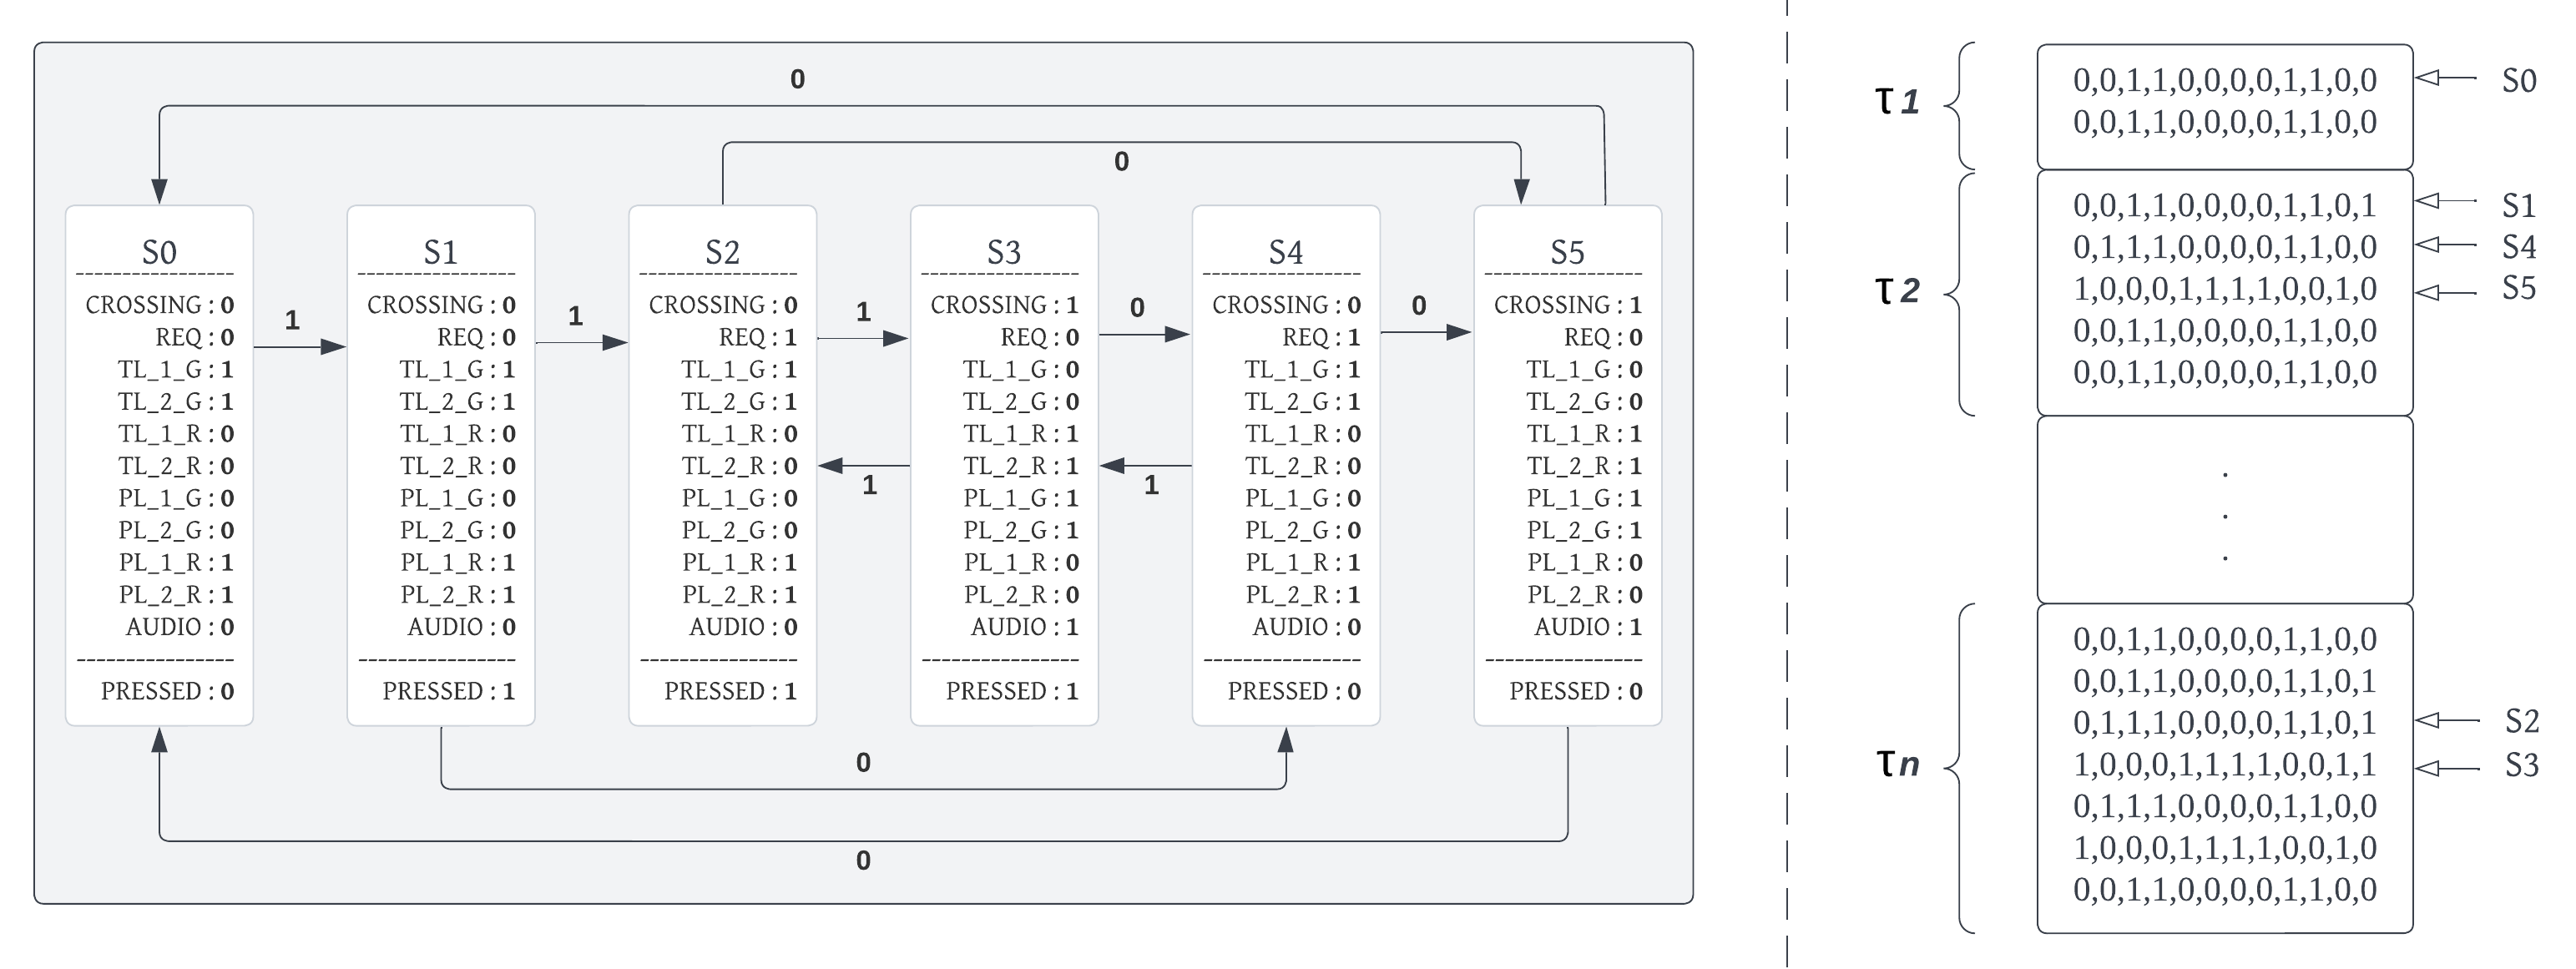
\includegraphics[width=\columnwidth]{figs/trajectory_stacks.png}
	\caption{Illustration of trajectory stacking from observation made during exploration of pelican crossing ladder logic program state space. Edge labels denote change in valuation of input variable PRESSED.}
\end{figure}

\subsection{Agent Implementation}
Here we introduce the network architecture used to train our RL agents. All algorithms presented in this work share the same architecture, adapting the input and output layers according to the environment. Our network input layer consists of $|Val_C \cup Val_I|$ nodes for given ladder logic formula $\psi$. Similarly, the output layer, responsible for mapping observations to the action space, comprises $|Val_I|$ nodes. All networks include a single fully connected hidden layer as this was empirically shown to produce the best performance. Learning rates for DQN, A2C, A3C and PPO algorithms were tuned individually according to the environment, falling within the range [0.0001, 0.001]. RMSProp was used to optimise the objective function. 

\section{Results}\label{sec:results}
\subsection{Environment Generation} 
Given exhaustive search of large state spaces is often computationally intractable, we have generated a set of ladder logic programs where the number of reachable states and depth are known. This enables us to analyse the performance of our approach on state spaces with known ground truths. Using existing models of ladder logic structures as a base environment template~\cite{james2013verification}, we derive progressively larger programs by sequentially introducing additional rungs. This way a predictable growth pattern is devised. Where $|S(\psi_i)|$, represents the number of reachable states for a program $\psi_i$, a subsequently generated program $\psi_{i+1}$ with one additional rung, has $2|S(\psi_i)|+1$ reachable states. During interaction with each environment we record the number of states observed by agents to gauge the overall state space coverage.

 \todo{Add fig: pelican state space highlighting gated condition holding for S0, branching off to an extended space}
 \todo{Highlight intended depth effect in correlation time series w.r.t ACT\_max}

%The following algorithm modifies the body of a pelican crossing ladder logic program given in Section~\ref{sec:ladder_logic}. For every $i^{th}$ rung introduced to lengthen the base program, we define two additional variables, VAR\_$i$ and ACT\_$i$. This effectively doubles the existing state space, increases the size of each state observation and introduces as increments the size of $\mathcal{A}$ by 2.
%\begin{figure}[!h]
%	\begin{algorithmic}\label{algo:ladder_generation}
%		\Procedure{Generate Ladder}{$n\_rungs$, $prog$}
%		\State cond $\gets$ ($\lnot$ PRESSED $\land$ $\lnot$CROSSING) $\land$ $\lnot$ REQ)
%		\State rung $\gets$ ACT\_1 $\land$ cond
%		\State coil $\gets$ VAR\_1 $\leftrightarrow$ rung
%		\State $i \gets 1$ 
%		\While{$i \leq$ n\_rungs}
%		\State $i \gets i+1$
%		\State new\_rung $\gets$ ACT\_[i] $\land$ (rung)
%		\State new\_coil $\gets$ VAR\_[i] $\leftrightarrow$ (new\_rung)
%		\State \textbf{append} new\_coil \textbf{to} $prog$
%		\EndWhile
%		\State \textbf{return} $prog$
%		\EndProcedure
%	\end{algorithmic}
%	\caption{Algorithm for automatic generation of ladder logic programs with controlled state space inflation.}
%	\label{fig:algorithm}
%\end{figure}

%Figure \ref{fig:state_space} was generated using the additional rung:
%\begin{align*}
%	VAR\_1 = ACT\_1 \land (\lnot PRESSED) \land \\(\lnot CROSSING) \land (\lnot REQ)
%\end{align*}
%Applying the above algorithm with $n\_rungs=0$ produces the complete state space of Figure~\ref{fig:state_space}. For readability and illustration we have obfuscated three states from the original ladder logic program in Section \ref{sec:ladder_logic}, abstracted as the `Pelican State Space'. Similarly, five states and their connected transitions are abstracted as the `Extended State Space'.  Again, dashed edges between states denote transitions induced by actions we have introduced while hard lined edges represent actions induced by valuations of the original input variable PRESSED. Transition labels from the LTS are highlighted in blue, while action selection according to the RL agent is shown in red. 
Results presented in Section~\ref{sec:results} are based on a set of generated programs ranging from $2^{14}$ to $2^{50}$ states\footnote{We note that interlocking programs generate much larger state spaces for model checking. However, work on abstractions by James et al.~\cite{james2011automatically} have shown that the state space can be reduced, in many cases, to an approximate size of $2^{50}$}, referenced in Table~\ref{tab:a3c_results}.

\todo{Add fig: illustration of stacked trajectories}
%\begin{figure*}[!t]
%	\centering
%	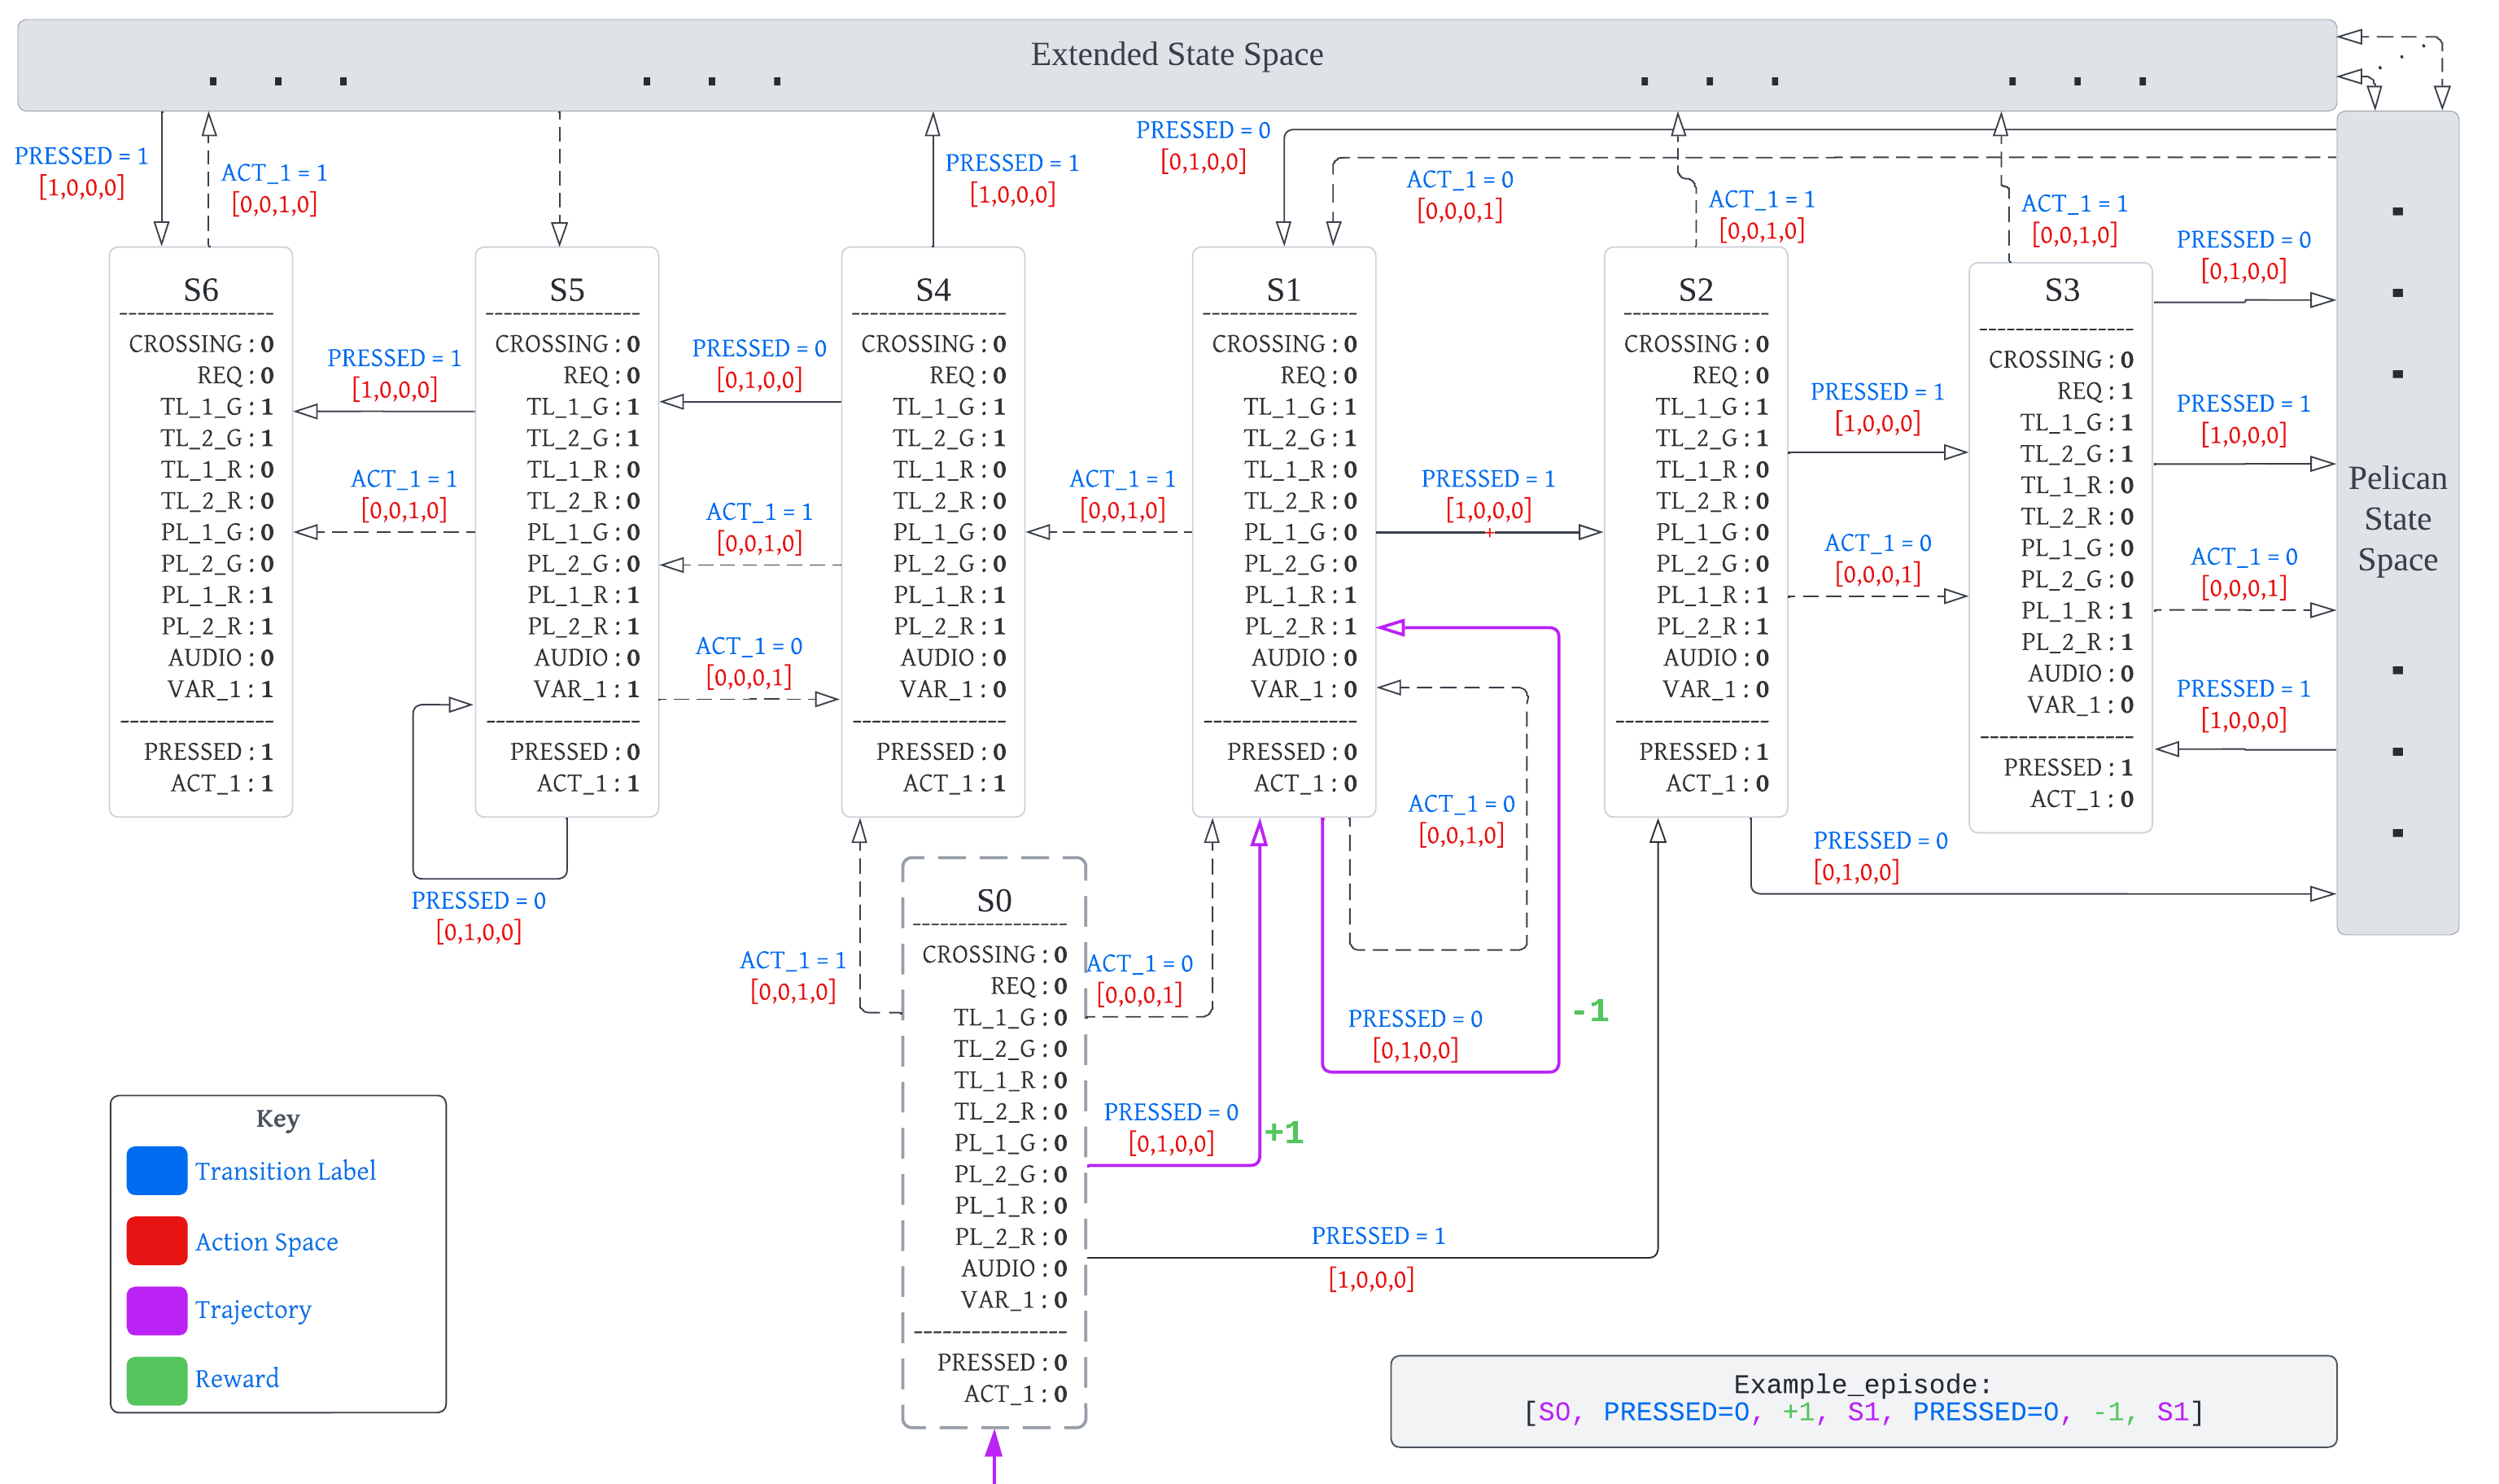
\includegraphics[width=\linewidth]{figs/pelican_states.png}
%	% where an .eps filename suffix will be assumed under latex, 
%	% and a .pdf suffix will be assumed for pdflatex; or what has been declared
%	% via \DeclareGraphicsExtensions.
%	\caption{Simplified state space representation of generated ladder logic program with one additional input variable ACT\_1 and one output coil VAR\_1.}
%	\label{fig:state_space}
%\end{figure*}

\subsection{State Space Coverage}
Preliminary results applying the A3C algorithm to a number of generated programs are outlined in Table \ref{tab:a3c_results}. Training was distributed among 32 CPU worker threads. `Actions' referenced in the third column refer to the number of possible assignments over input variables in each ladder program, from every state. Depth, the first agent column, refers to the greatest number of steps taken before repeating observations in the environment, across all workers.

Coverage metrics are expectedly maximised for environments with a small number of reachable states with acceptable levels of coverage for programs with a theoretical size up to $2^{40}$. Interestingly, we observed longer training durations without early stopping occasionally increased coverage beyond a certain threshold. It is possible workers learn an optimal search strategy within a subregion of the state space. Additionally, performance in terms of max depth and states reached increased by approx. $5\%$ when decreasing the total number of episodes from $3 \times 10^{5}$ to $1.5\times10^{5}$ episodes. This may be a product of random episode initialisation spawning workers in more desirable states where stochastic action sampling happened to lead to unfamiliar subregions of the environment.

Performance in terms of cumulative reward which failed to maximise coverage often increased linearly before collapsing to some suboptimal reward. This may be due to tendencies for large network updates to shift the network gradients into a bad local minima, from which performance does not recover within the allotted training duration. The on-policy nature of actor critic means trajectories generated via an old policy are no longer sampled during minibatch updates for the current policy, thus biasing behaviour to the most recent model updates and introducing sample inefficiency. Adding on policy memory strategies\cite{wang2017sample} may help avoid this in future applications

Given the A3C algorithm requires workers to asynchronously update their shared network every $T_{\max}$ steps or on episode termination, larger values for $T_{\max}$ consolidate more information regarding worker trajectories before applying gradient updates to their local network. We found the most significant improvements to performance in terms of coverage metrics and increasing the $k$ bound when introducing workers to larger environments, was lower update frequencies and random start state initialisation. Prior to these adjustments workers, irrespective of their number, seldom covered 80\% of most smaller environments. Similarly, for the largest environment with $2^{50}$ states, coverage improved from 3.2\% to 41.48\%

\begin{table}[!h]
	\caption{A3C Coverage Metrics}
	\label{tab:a3c_results}
	\centering
	\begin{tabular}{rrrrr}
		\hline
		\multicolumn{3}{c|}{Environment}                                                                                                                                                                     & \multicolumn{2}{c}{Agent}                                \\ \hline
		\multicolumn{1}{c}{\begin{tabular}[c]{@{}c@{}}States\\ (Theoretical)\end{tabular}} & \multicolumn{1}{c}{\begin{tabular}[c]{@{}c@{}}States\\ (Reachable)\end{tabular}} & \multicolumn{1}{c|}{Actions} & \multicolumn{1}{c}{Depth} & \multicolumn{1}{c}{Coverage} \\ \hline
		\rowcolor[HTML]{FFFFFF} 
		$2^{14}$                                                              & 15                                                                               & 2                            & 14                        & 100.0                          \\
		\rowcolor[HTML]{FFFFFF} 
		$2^{16}$                                                              & 31                                                                               & 4                            & 28                        & 100.0                          \\
		\rowcolor[HTML]{FFFFFF} 
		$2^{18}$                                                             & 63                                                                               & 6                            & 48                        & 100.0                          \\
		\rowcolor[HTML]{FFFFFF} 
		$2^{20}$                                                             & 127                                                                              & 8                            & 33                        & 100.0                          \\
		\rowcolor[HTML]{FFFFFF} 
		$2^{22}$                                                              & 255                                                                              & 10                           & 76                        & 100.0                          \\
		\rowcolor[HTML]{FFFFFF} 
		$2^{24}$                                                              & 511                                                                              & 12                           & 49                        & 100.0                          \\
		\rowcolor[HTML]{FFFFFF} 
		$2^{26}$                                                             & 1023                                                                             & 14                           & 306                       & 100.0                          \\
		\rowcolor[HTML]{FFFFFF} 
		$2^{28}$                                                              & 2047                                                                             & 16                           & 538                       & 100.0                          \\
		\rowcolor[HTML]{FFFFFF} 
		$2^{30}$                                                              & 4095                                                                             & 18                           & 1418                      & 99.731                       \\
		\rowcolor[HTML]{FFFFFF} 
		$2^{32}$                                                              & 8191                                                                             & 20                           & 1712                      & 96.532                       \\
		\rowcolor[HTML]{FFFFFF} 
		$2^{34}$                                                              & 16383                                                                            & 22                           & 1498                      & 95.550                       \\
		\rowcolor[HTML]{FFFFFF} 
		$2^{36}$                                                              & 32767                                                                            & 24                           & 2879                      & 84.694                       \\
		\rowcolor[HTML]{FFFFFF} 
		$2^{38}$                                                              & 65535                                                                            & 26                           & 1969                      & 89.071                       \\
		\rowcolor[HTML]{FFFFFF} 
		$2^{40}$                                                              & 131071                                                                           & 28                           & 2692                      & 82.884                       \\
		\rowcolor[HTML]{FFFFFF} 
		$2^{42}$                                                              & 262143                                                                           & 30                           & 1406                      & 76.033                       \\
		\rowcolor[HTML]{FFFFFF} 
		$2^{44}$                                                              & 524287                                                                           & 32                           & 1782                      & 62.137                       \\
		\rowcolor[HTML]{FFFFFF} 
		$2^{46}$                                                              & 1048575                                                                          & 34                           & 1593                      & 64.053                       \\
		\rowcolor[HTML]{FFFFFF} 
		$2^{48}$                                                              & 2097151                                                                          & 36                           & 1598                      & 57.547                       \\
		\rowcolor[HTML]{FFFFFF} 
		$2^{50}$                                                              & 4194303                                                                          & 38                           & 2566                      & 41.483                       \\ \hline
	\end{tabular}
\end{table}

\subsection{Variable Correlation}

Phi coefficients are computed to show the association between a pair of binary variables. Values range $[-1,1]$ where $1$ is complete correlation and $-1$ is an inverse relation.  

\begin{figure}[!t]
	\label{fig:heatmap}
	\centering
	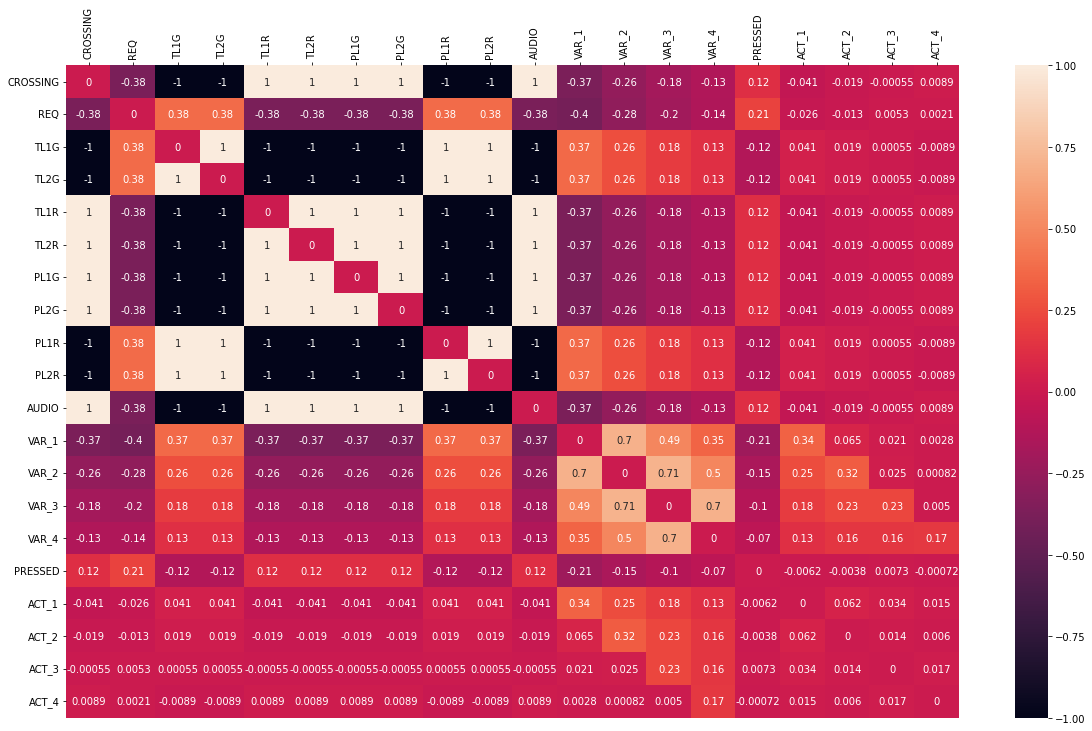
\includegraphics[width=\columnwidth]{figs/heatmap.png}
	\caption{Correlation matrix for ladder logic program with four additional synthetically generated rungs, 127 reachable states and $2^{20}$ theoretical states.}
\end{figure}


Consider Figure \ref{fig:heatmap}. Computing the phi coefficients for a set of binary variables from a generated ladder logic program with $2^{20}$ theoretical states, produces a symmetric $N\times N$ matrix, where element $m_{0,1}$ refers to the phi coefficient between $CROSSING$ and $REQ$. Entries computing self correlation are read on the diagonal, and have been set to $0$. $\phi$ coefficients require an empirical sample of observations in order to reveal any correlation. Naturally, the more unique samples concerning the binary variables under evaluation produce more accurate estimates of their relation. Given we wish to learn relations over massive state spaces it is likely our agent's begin with a noisy estimate of variable correlation without observing the majority of states, i.e without knowledge of all variable configurations under the reachable states, $\phi$ will remain an approximation (isn't it anyway?). 

Immediately we notice certain aspects of program semantics, particularly variable assignment conditions, from Figure \ref{fig:heatmap}. Upper left quadrant represents base pelican crossing program. See strong positive and inverse correlation between variables responsible for traffic and pedestrian control during crossing procedures. Expectedly, green aspects for traffic $TL\_1\_G, TL\_2\_G$ are inversely related to green aspects for pedestrians, i.e both sets of lights should not simultaneously indicate a safe advance (Is this the invariant?). From this we can infer our own trivial invariant property given this relation is never explicitly defined in the program given all values for light aspects are assigned using the present value of $CROSSING$.

\todo{Add fig: correlation time series (w.r.t a variable subset)}

Figure \ref{fig:phi_timeseries} demonstrates the convergence of phi over training time steps, each plot illustrating correlation with respect to a single variable under evaluation. Lines fixed at $0$ represent the variable under evaluation, ignoring self correlation. Lines fixed at $1$ or $-1$ are variables positively or inversely related to the variable under evaluation. Note during earlier timesteps, estimates of phi are volatile until sufficient state space coverage stabilises the number of samples used in computing $\phi$. We see for small programs, these values converge quickly as the number of reachable states are low. For larger programs we would expect greater variability in correlation as our RL agents take longer to sufficiently populate $A_\tau$ with new observations. $\phi$ coefficients fluctuating between no relation and one of the extremes may suggest insufficient exploration of states 


\subsubsection{Reward Shaping}
\todo{Discuss optimising phi coeffs to converge over time.}

\subsection{Use of mining to validate generated data}
\todo{Highlight generated program / artificially depth}
In generating ladder logic programs to serve as training environments we introduce a condition $VAR\_1 = ACT\_1 \land (\lnot CROSSING) \land \lnot REQ \land PRESSED)$, which only holds for $S1$ of the original pelican crossing. Subsequent rungs build upon this condition for every additional $ACT\_N$ and $VAR\_N$, ensuring every $n^th$ action introduced increases the overall state space depth. We would then expect ACT$\_1$,...,ACT$\_N$ to be correlated.  
Observing the lower right quadrant of Figure \ref{fig:heatmap} we see properties of our program generation in how additional actions and variables become less related to our original program state space.   

\subsection{Trajectory Clustering}

%We now present a set of results from applying our approach to a series of generated ladder logic programs, modelled as learning environments. The following section is divided into three parts, first discussing the merits and drawbacks of the respective learning algorithms. Second, we present results from applying the multi agent A3C algorithm to our full set of generated ladder logic programs, shown in Table \ref{tab:a3c_results}. Finally we discuss performance differences between single agent implementations of A2C and PPO, as they exhibited divergent learning objectives.
%
%
%\subsection{Algorithmic Trends}\label{sec:algorithmic_trends}
%
%Initially, to test our model, we train a simple DQN agent on a set of generated programs, up to $2^{20}$ theoretic states and 127 reachable. The agent often observes complete state coverage within the time taken for the more advanced A2C and PPO algorithms to determine state space depth. DQNs exhibited difficulty scaling well to state space depth learning objective without significant hyperparameter tuning, failing to converge performance on the smallest environments. It is likely using DQN without a prioritised replay buffer~\cite{andrychowicz2017hindsight} leads to poor training sample efficiency when applying network updates. We expect agents exploring ladder logic program states to rarely observe the greatest depth, meaning episodes resulting in optimal rewards may never be sampled for training. Bootstrapping the action-value function via a target network also introduces an additional challenge in selecting an update interval frequent enough to avoid overestimating state-action values. Similarly, the use of replay memory requires an initial training delay to populate the buffer before Q-Network updates. Setting the gradient step size is likely dependent on the  learnable function complexity, which is expected to increase with environment size. The off-policy nature of DQNs constrains network updates with trajectories produced under other, presumably less optimal, policies. Governing the DQN exploration rate explicitly using an $\epsilon$-greedy strategy seems unstable given this could reduce random action exploration with large subregions of an environment unobserved. While DQN demonstrates the potential of RL algorithms in learning policies for prediction and control, they are unlikely to scale sufficiently to interlocking state spaces for the purposes of invariant finding.
%
%Two Actor critic methods, single agent Advantage Actor-Critic (A2C) and its asynchronous multi-agent counterpart (A3C) are applied to all 19 generated environments. Having several workers and an on-policy learning algorithm removes need of replay memory and any training delay to accumulate sufficient experience. Actor and critic networks, approximating the behaviour policy and value function, provide better convergence guarantees at the cost of some additional complexity in learned parameters. Paired with randomised reset logic both algorithms accumulate experience faster than conventional DQN, achieving good coverage on a range of medium to large state spaces.  Actor-critic algorithms, while improved by more informed value estimation and policy iteration, are also susceptible to performance collapse in sufficiently complex environments or over long training periods. Parameter updates have a tendency to push the policy  into an unfamiliar region of policy space from which subsequent updates are unable to recover, potentially `collapsing' the model. Unsurprisingly, A3C outperforms the single agent variant and shows the best coverage metric among all policy gradient methods applied. A3C and its results are discussed in depth in Section~\ref{sec:asynch}.
%
%It is for this reason we move to Proximal Policy Optimisation (PPO), to constrain the magnitude of gradient steps during the parameter update. It is our expectation that limiting policy, and potentially value function, updates within a clip range~\cite{schulman2017proximal} or according to KL-divergence between the current and most recent policy~\cite{schulman2017trust}, making the model more resilient to collapse. Trust region methods generally require fewer hyperparameter adjustments being more stable learning strategies. We observe this in Section~\ref{sec:trust_regions}, where PPO demonstrates slow but linear state exploration while appearing to maximise state depth within a known subregion.
%
%\subsection{Asynchronous Exploration}\label{sec:asynch}
%\begin{table}[!t]
%	\caption{A3C Coverage Metrics}
%	\label{tab:a3c_results}
%	\centering
%	\begin{tabular}{rrrrr}
%		\hline
%		\multicolumn{3}{c|}{Environment}                                                                                                                                                                     & \multicolumn{2}{c}{Agent}                                \\ \hline
%		\multicolumn{1}{c}{\begin{tabular}[c]{@{}c@{}}States\\ (Theoretical)\end{tabular}} & \multicolumn{1}{c}{\begin{tabular}[c]{@{}c@{}}States\\ (Reachable)\end{tabular}} & \multicolumn{1}{c|}{Actions} & \multicolumn{1}{c}{Depth} & \multicolumn{1}{c}{\begin{tabular}[c]{@{}c@{}-0.987531}Coverage (\%) \\ reachable states\end{tabular}} \\ \hline
%		\rowcolor[HTML]{FFFFFF} 
%		$2^{14}$                                                              & 15                                                                               & 2                            & 14                        & 100.0                          \\
%		\rowcolor[HTML]{FFFFFF} 
%		$2^{16}$                                                              & 31                                                                               & 4                            & 28                        & 100.0                          \\
%		\rowcolor[HTML]{FFFFFF} 
%		$2^{18}$                                                             & 63                                                                               & 6                            & 48                        & 100.0                          \\
%		\rowcolor[HTML]{FFFFFF} 
%		$2^{20}$                                                             & 127                                                                              & 8                            & 33                        & 100.0                          \\
%		\rowcolor[HTML]{FFFFFF} 
%		$2^{22}$                                                              & 255                                                                              & 10                           & 76                        & 100.0                          \\
%		\rowcolor[HTML]{FFFFFF} 
%		$2^{24}$                                                              & 511                                                                              & 12                           & 49                        & 100.0                          \\
%		\rowcolor[HTML]{FFFFFF} 
%		$2^{26}$                                                             & 1023                                                                             & 14                           & 306                       & 100.0                          \\
%		\rowcolor[HTML]{FFFFFF} 
%		$2^{28}$                                                              & 2047                                                                             & 16                           & 538                       & 100.0                          \\
%		\rowcolor[HTML]{FFFFFF} 
%		$2^{30}$                                                              & 4095                                                                             & 18                           & 1418                      & 99.731                       \\
%		\rowcolor[HTML]{FFFFFF} 
%		$2^{32}$                                                              & 8191                                                                             & 20                           & 1712                      & 96.532                       \\
%		\rowcolor[HTML]{FFFFFF} 
%		$2^{34}$                                                              & 16383                                                                            & 22                           & 1498                      & 95.550                       \\
%		\rowcolor[HTML]{FFFFFF} 
%		$2^{36}$                                                              & 32767                                                                            & 24                           & 2879                      & 84.694                       \\
%		\rowcolor[HTML]{FFFFFF} 
%		$2^{38}$                                                              & 65535                                                                            & 26                           & 1969                      & 89.071                       \\
%		\rowcolor[HTML]{FFFFFF} 
%		$2^{40}$                                                              & 131071                                                                           & 28                           & 2692                      & 82.884                       \\
%		\rowcolor[HTML]{FFFFFF} 
%		$2^{42}$                                                              & 262143                                                                           & 30                           & 1406                      & 76.033                       \\
%		\rowcolor[HTML]{FFFFFF} 
%		$2^{44}$                                                              & 524287                                                                           & 32                           & 1782                      & 62.137                       \\
%		\rowcolor[HTML]{FFFFFF} 
%		$2^{46}$                                                              & 1048575                                                                          & 34                           & 1593                      & 64.053                       \\
%		\rowcolor[HTML]{FFFFFF} 
%		$2^{48}$                                                              & 2097151                                                                          & 36                           & 1598                      & 57.547                       \\
%		\rowcolor[HTML]{FFFFFF} 
%		$2^{50}$                                                              & 4194303                                                                          & 38                           & 2566                      & 41.483                       \\ \hline
%	\end{tabular}
%\end{table}
%
%Preliminary results applying the A3C algorithm to a number of generated programs are outlined in Table \ref{tab:a3c_results}. Training was distributed among 32 CPU worker threads. `Actions' referenced in the third column refer to the number of possible assignments over input variables in each ladder logic program, from every state. Depth, the first agent column, refers to the greatest number of (loop free) steps observed across all workers, within a single episode.
%
%Coverage metrics are expectedly maximised for environments with a small number of reachable states with acceptable levels of coverage for programs with a theoretical size up to $2^{40}$. Interestingly, we observed longer training durations without early stopping occasionally increased coverage beyond a certain threshold. It is possible workers learn an optimal search strategy within a subregion of the state space. Additionally, performance in terms of max depth and states reached increased by approximately $5\%$ when decreasing the total number of episodes from $3 \times 10^{5}$ to $1.5\times10^{5}$ episodes. This may be a product of random episode initialisation spawning workers in more desirable states where stochastic action sampling happened to lead to unfamiliar subregions of the environment.
%
%Performance in terms of cumulative reward which failed to maximise coverage often increased linearly before collapsing to some suboptimal reward. This may be due to tendencies for large network updates to shift the network gradients into a bad local minima, from which performance does not recover within the allotted training duration. The on-policy nature of actor critic means trajectories generated via an old policy are no longer sampled during gradient updates for the current policy, thus biasing behaviour to the most recent model updates and introducing sample inefficiency. Adding on policy memory strategies\cite{wang2017sample} may help avoid this in future applications.
%
%Given the A3C algorithm requires workers to asynchronously update their shared network every $T_{\max}$ steps or on episode termination, larger values for $T_{\max}$ consolidate more information regarding worker trajectories before applying gradient updates to their local network. We found the most significant improvements to performance in terms of coverage metrics and increasing the $k$ bound when introducing workers to larger environments, was lower update frequencies and random start state initialisation. Prior to these adjustments workers, irrespective of their number, seldom covered 80\% of most smaller environments. Similarly, for the largest environment with $2^{50}$ states, coverage improved from 3.21\% to 41.48\%
%
%\subsection{Trust Regions and Reward Shaping} \label{sec:trust_regions}
%
%\begin{figure*}[h]
%	\centering
%	\subfloat[Number of reachable states discovered during five hours of training.]{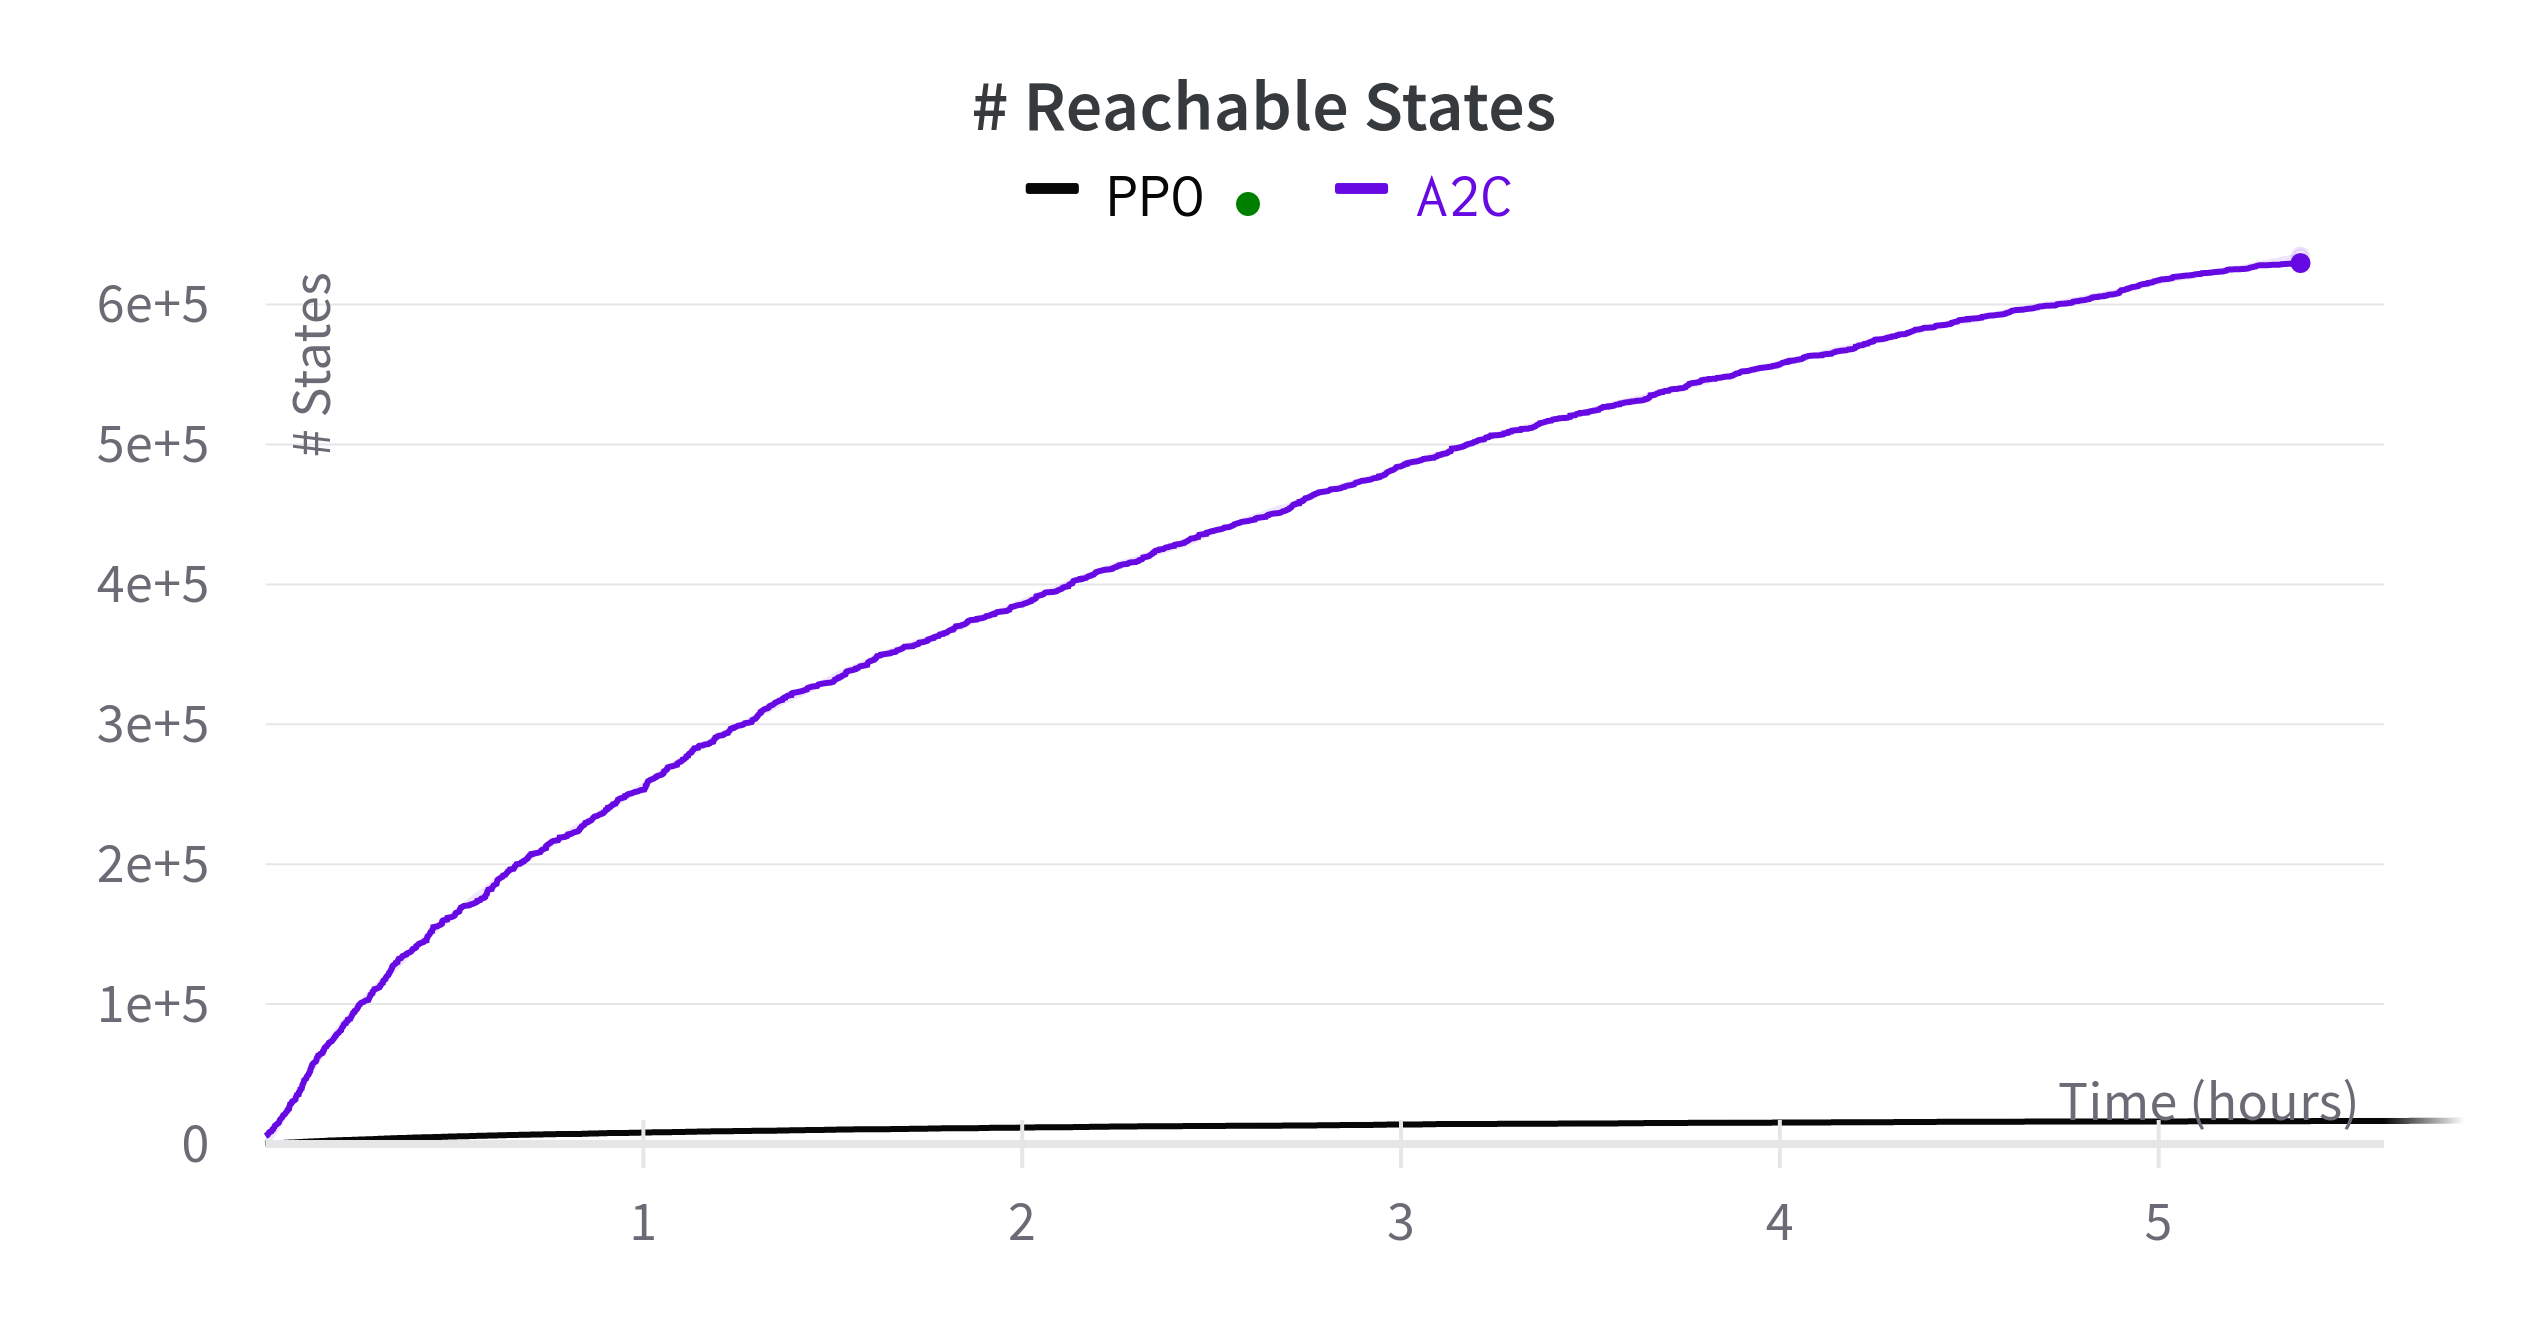
\includegraphics[width=2.5in]{figs/reachable_states.png}%
%		\label{fig_first_case}}
%	\subfloat[Max state space depth observed over 25 thousand training episodes.]{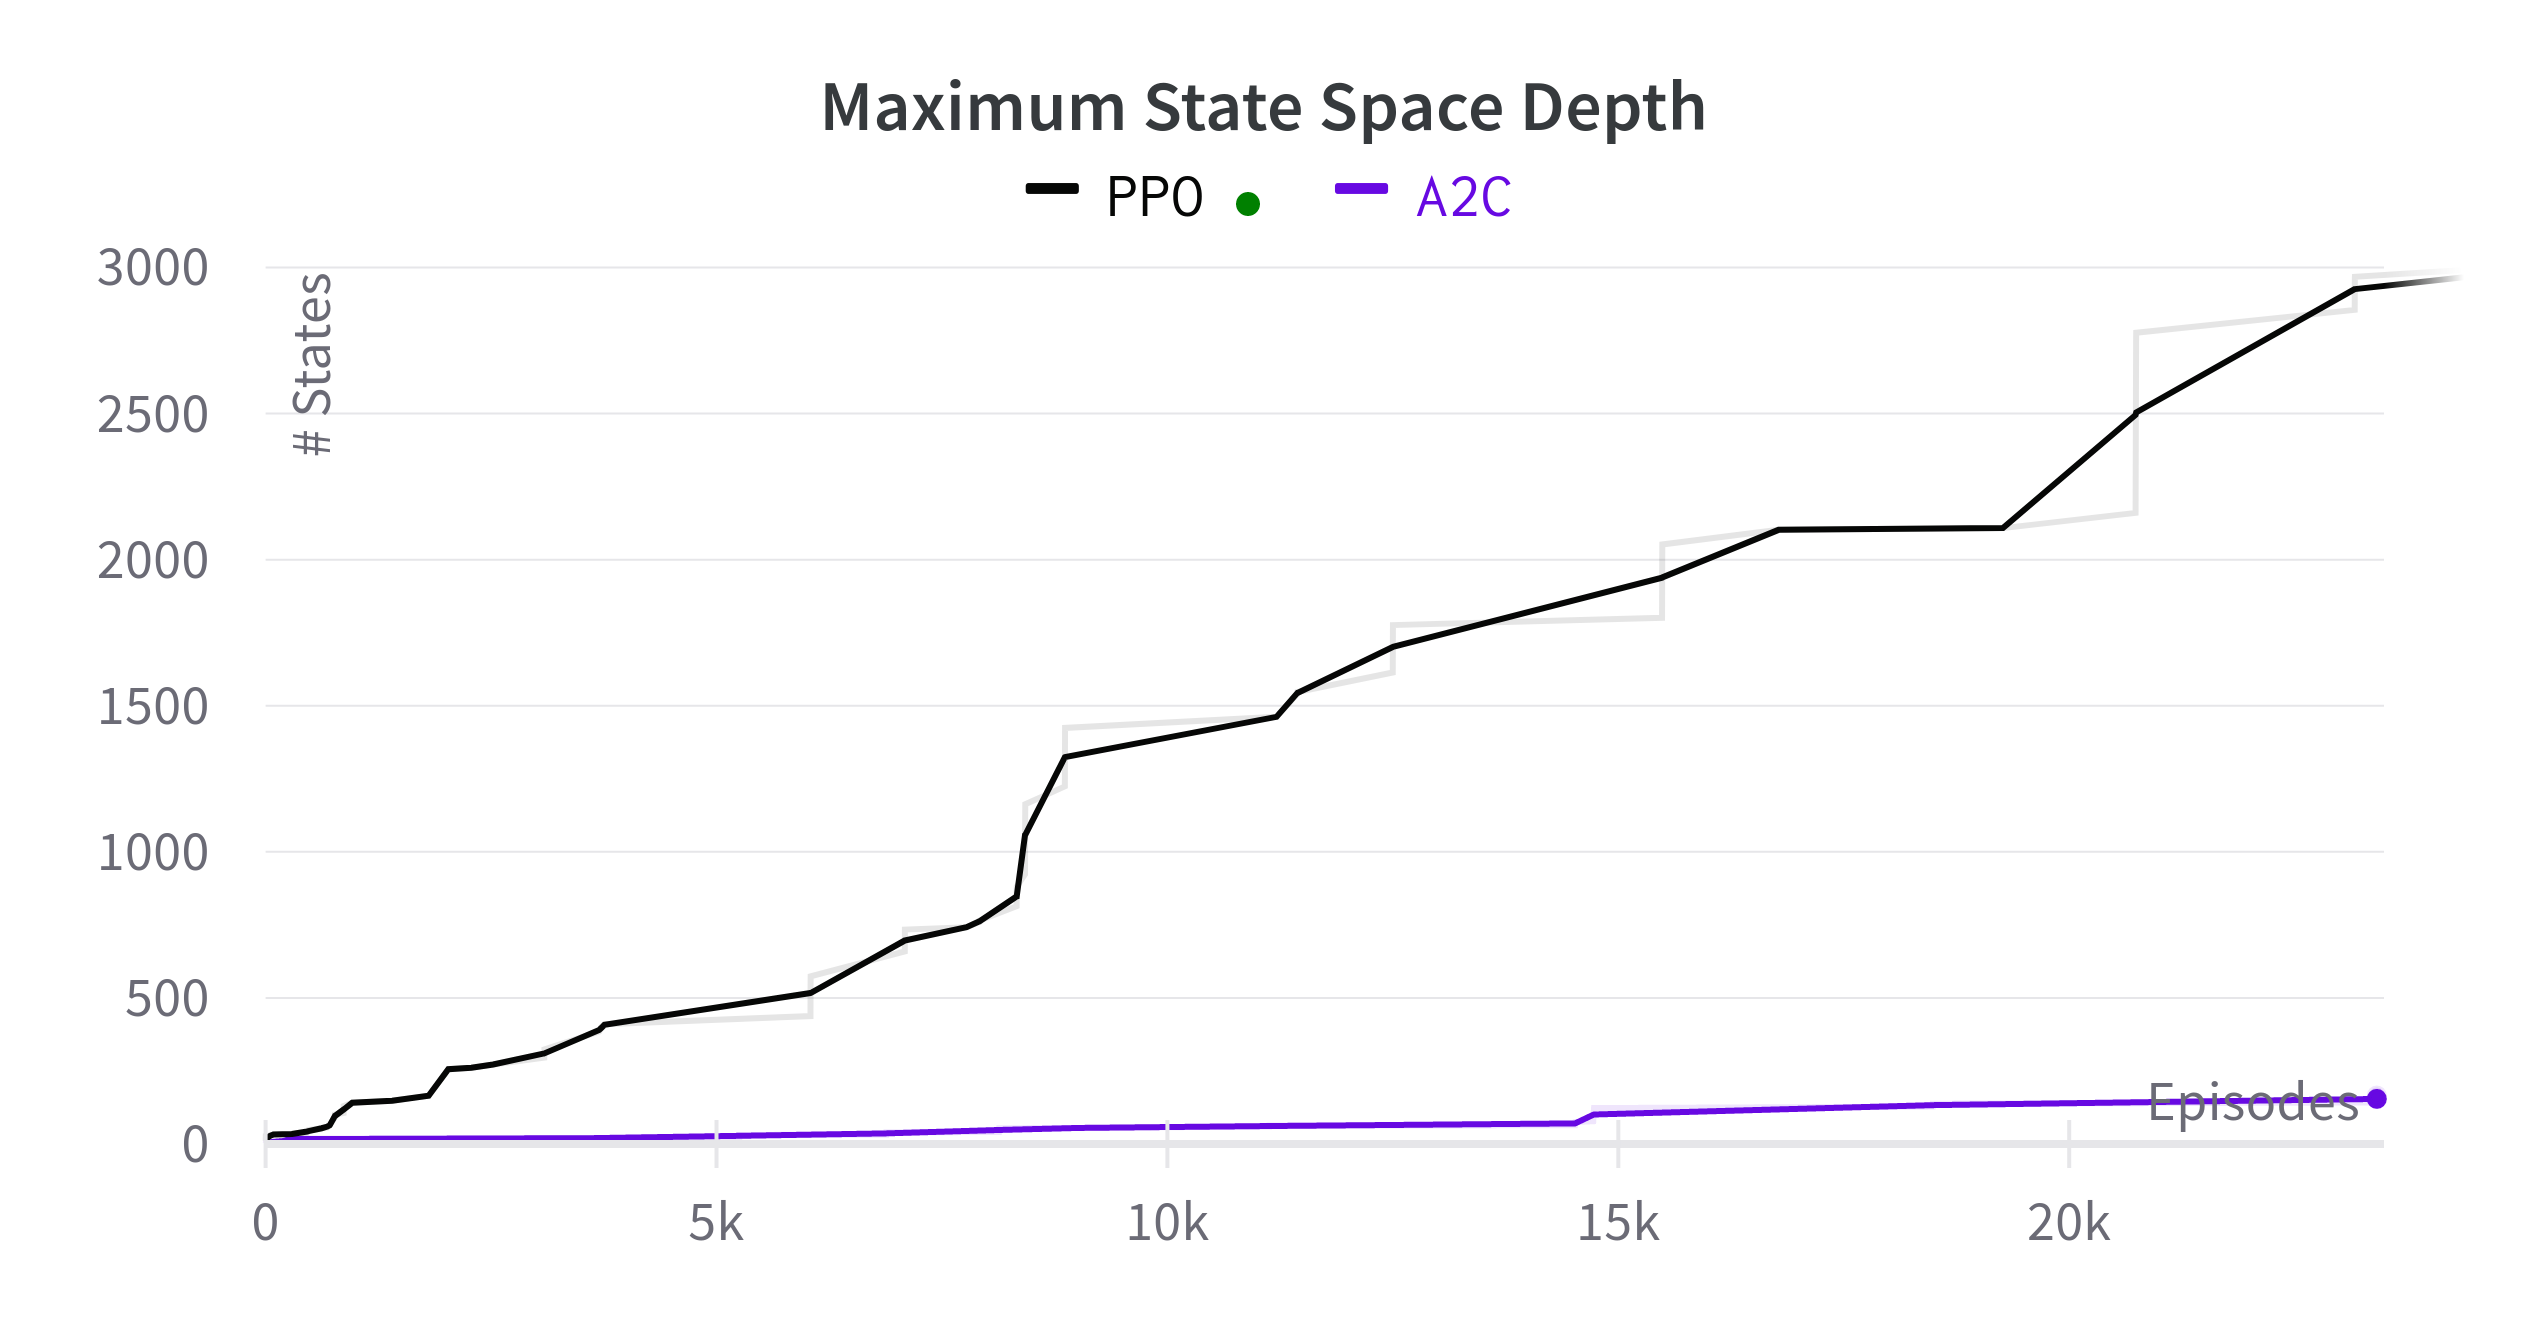
\includegraphics[width=2.5in]{figs/max_k.png}%
%		\label{fig_second_case}}
%	\hfil
%	\subfloat[Mean policy entropy loss. The negative average entropy output by the policy network.]{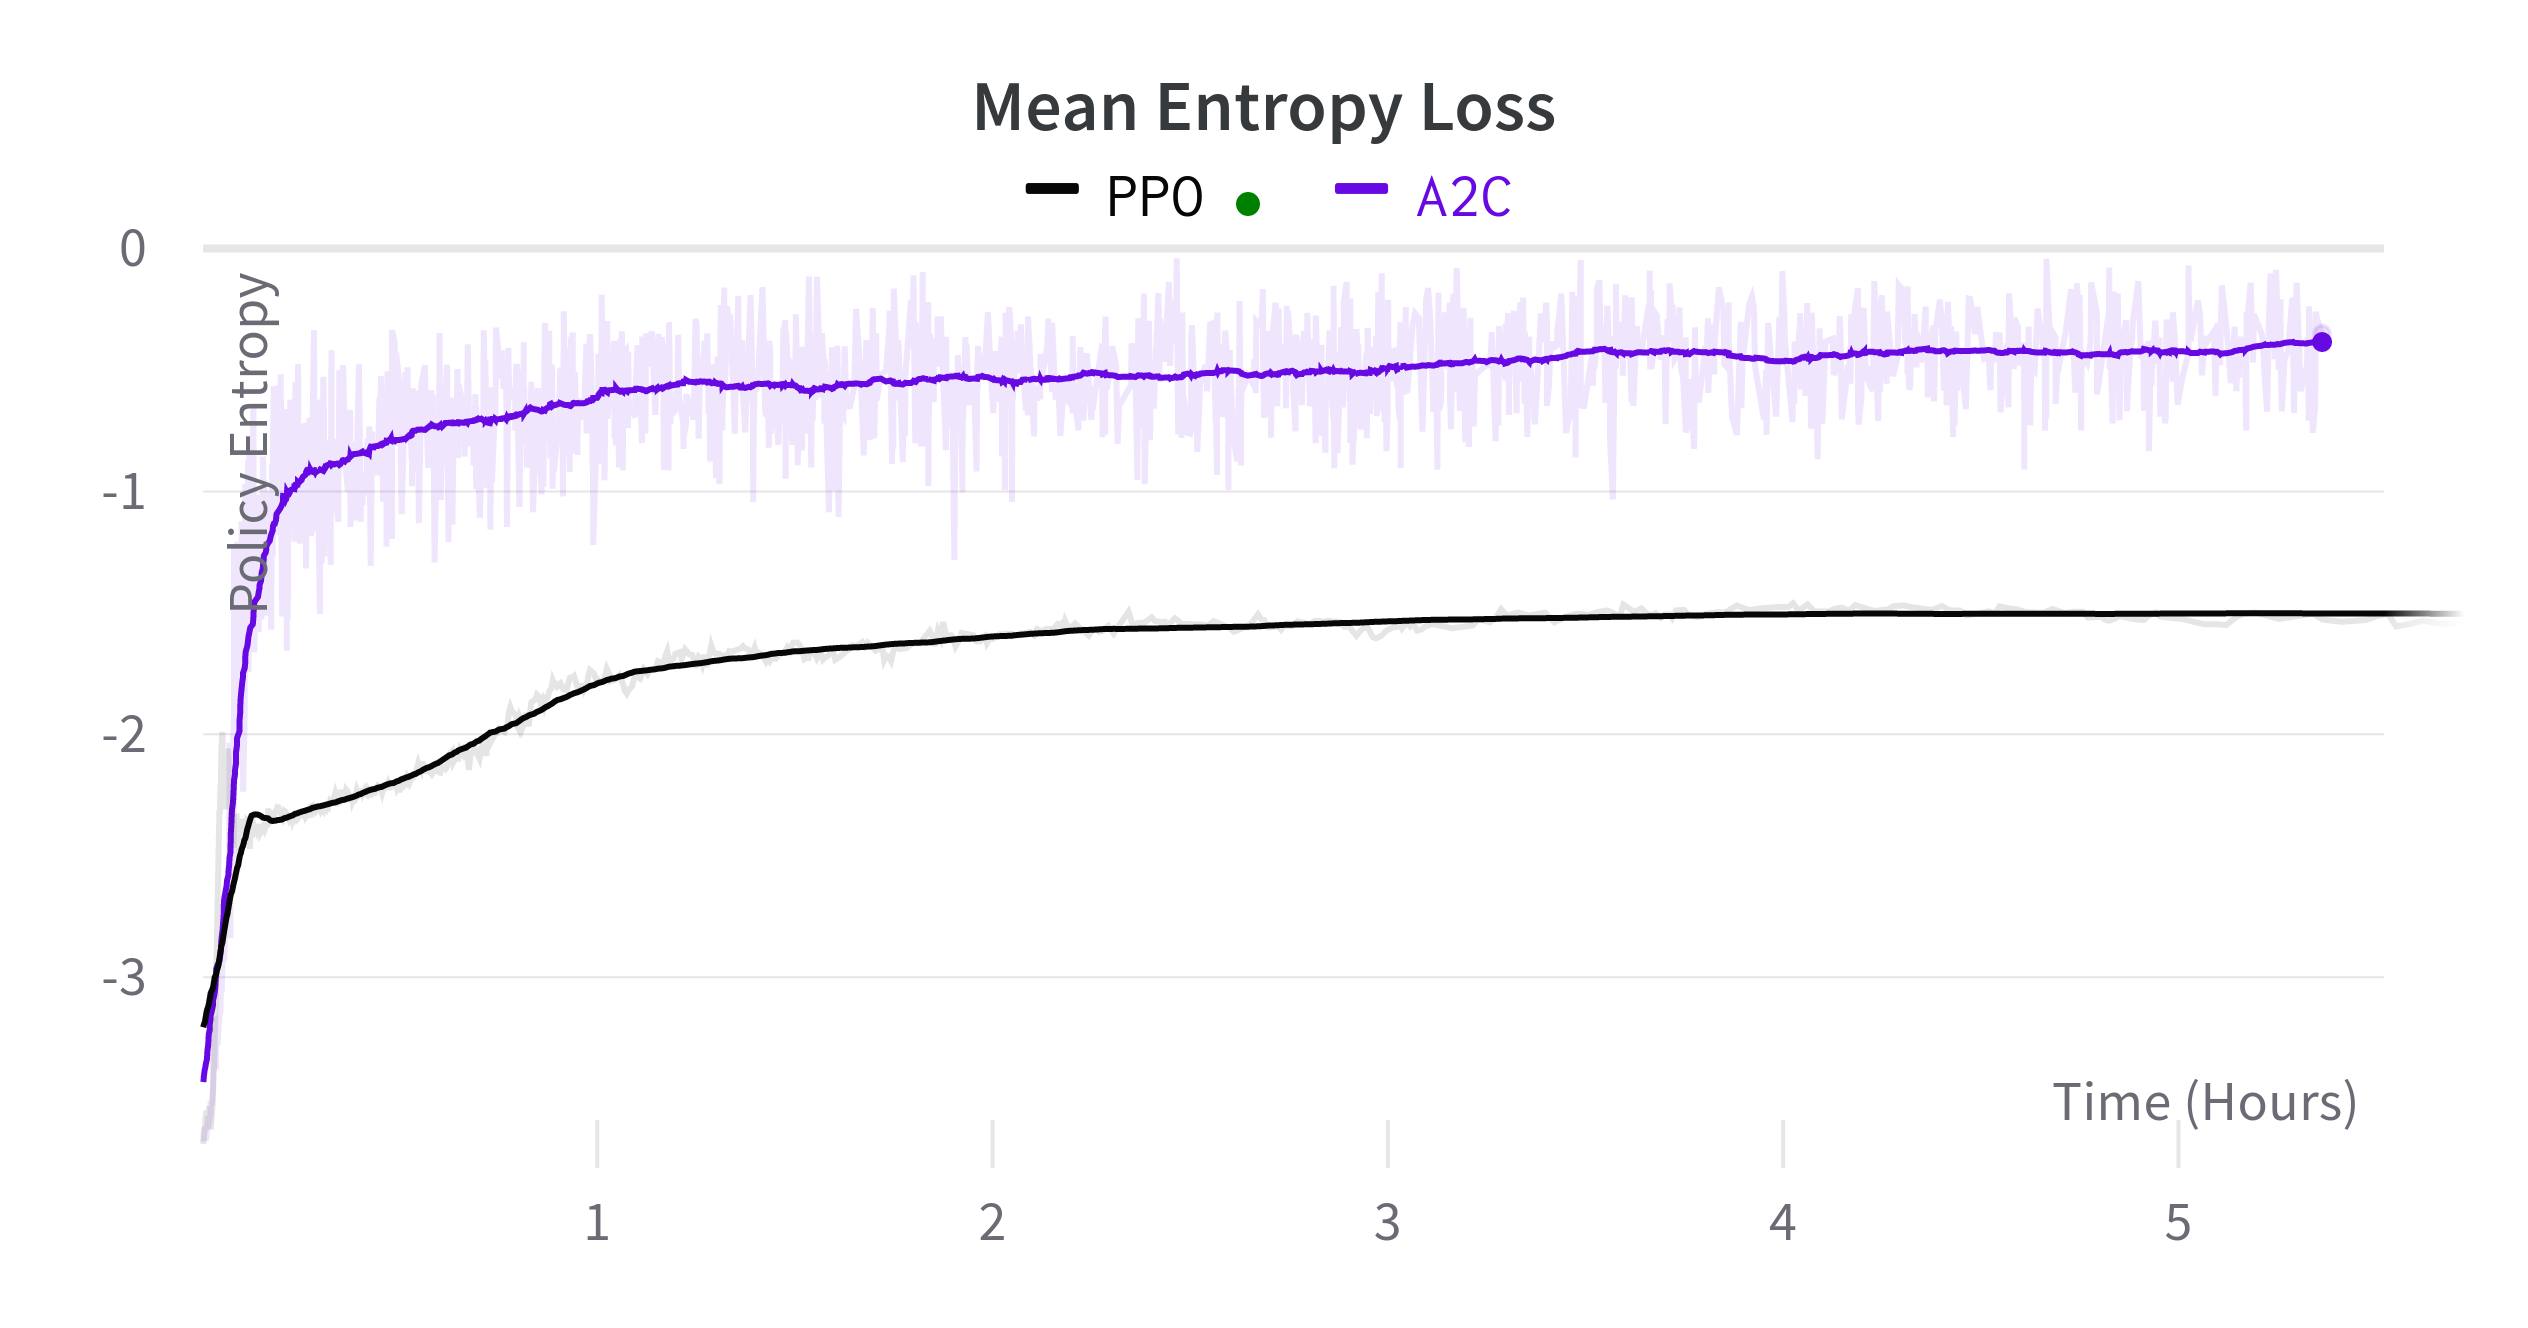
\includegraphics[width=2.5in]{figs/entropy.png}%
%		\label{fig_first_case}}
%	\subfloat[Rolling average of reward for 35 thousand training episodes.]{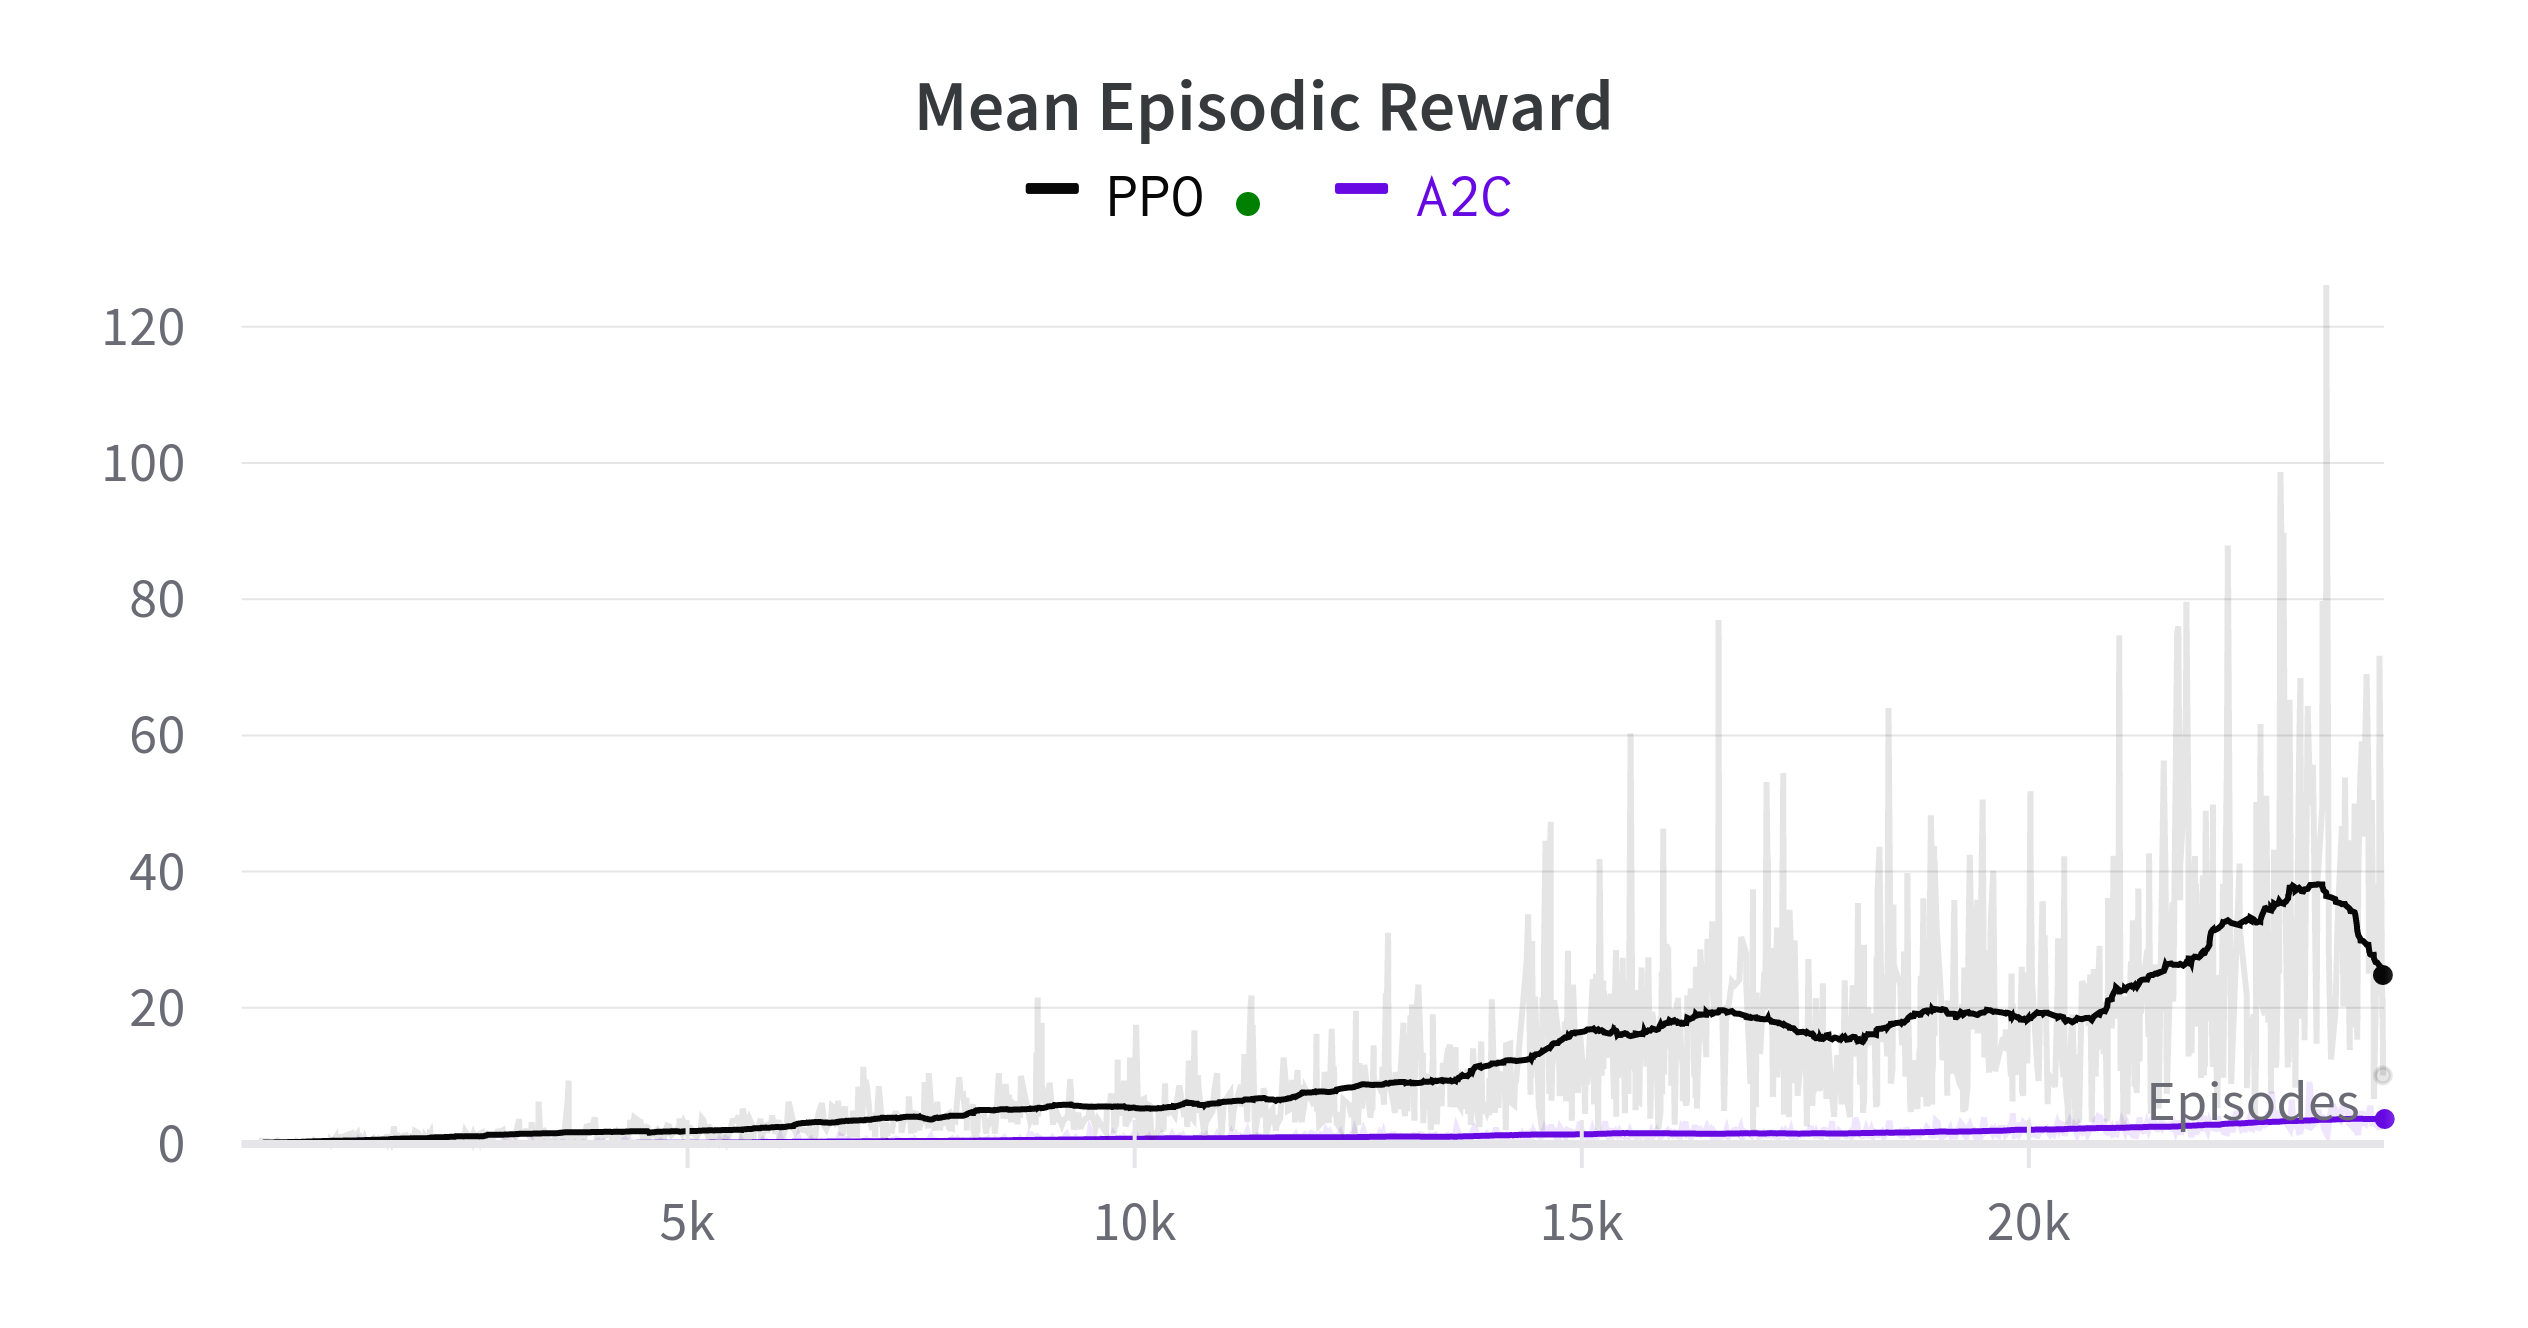
\includegraphics[width=2.5in]{figs/reward.png}%
%		\label{fig_second_case}}
%	\caption{Training and evaluation metrics during application of PPO and A2C algorithms on generated state space of a theoretic size $2^{50}$.}
%	\label{fig:performance}
%\end{figure*}
%
%Advantage actor critic methods seem to perform better in terms of coverage, particularly  distributed variants. The multi agent nature paired with no update clipping may allow for greater exploration at the cost of training stability. Having observed the best coverage performance from A3C, we select a number of ladder logic programs to compare single agent algorithms, namely A2C and PPO, in terms of their training behaviour and evaluation performance. Having designed our reward function as one of continued state novelty we expected PPO to outperform A2C, covering a greater proportion of states after A2C performance either plateaus or collapses.
%
%
%Figure~\ref{fig:performance}(a) shows the number of reachable state discovered by the agent during the first 5 hours of training on a ladder logic program with 19 additional rungs. A2C increases state coverage significantly faster than PPO but considering Figure~\ref{fig:performance}(b), struggles to learn which transitions reveal the max state depth within its discovered subregion.
%
%Again, Figure~\ref{fig:performance}(b) demonstrates PPO optimises better to the actual reward objective, maximising exploration of state-action pairs for the explored subregion while slowly increasing state coverage. The surrogate clipped objective used during the gradient update may contribute to how agents introduce new states by steadily exploring uncertain state-action pairs. Figure~\ref{fig:performance}(c) may also suggest this, in that we observe the mean entropy loss for PPO is significantly more stable than that of A2C, indicating the policy under PPO maintains higher levels of uncertainty. Conversely, A2C mean entropy loss appears to converge toward 0, indicating its predictions are more certain despite very poor performance in terms of the actual reward objective. Similarly the value function loss is more stable for PPO compared to A2C, this measures the temporal difference error (the deviation in prediction accuracy from its bootstrapped estimate) between the current value function and actual observed returns.
%
%Model performance across all learning algorithms appears sensitive to network update frequency and experience accumulation during rollout, prior to each update. This is certainly a property to be conscious of as it may translate interlocking programs, making this parameter dependent on the state space structure, where the total number of reachable states or longest acyclic path is unknown to us. Although, such efforts are not likely to pose an issue given the long development and testing cycles for interlockings. In future we would like to trial this set of algorithms, as well as some hybrid approaches~\cite{haarnoja2018soft}, using a modified reward function based on global state coverage or uncertainty maximisation.
%
%
%\section{Conclusion \& Future Work } 
%In this work, we have taken first steps towards using machine learning to generate invariants by providing a first formal mapping of interlocking based state spaces to a reinforcement learning environment. In addition, we have applied asynchronous and trust region deep reinforcement learning methods to programmatically generated state spaces and analysed their ability in terms of state coverage and state space depth. Our findings highlight that RL approaches can be successfully rewarded to explore a large percentage of a given state space in terms of state coverage, however that incentivising depth based exploration is more challenging. As any machine learning approach to finding invariants will likely need to explore such a state space these results show the credibility of such an approach. In our subsequent works we envisage the current learning framework to serve as a means of dataset generation, from which patterns or sequences of can be mined from agent trajectories. In particular, for mining invariants we hope to encode an embedding for agent trajectories and perform clustering on those batches of state sequences. Using a similarity measure, such as Manhattan or Euclidean distance~\cite{malkauthekar2013analysis}, we may be able to identify persistent features across regions of the state space, observed throughout training. The resulting clusters may indicate invariant properties present in the corresponding region of the explored state space. We envisage a number of data mining or sequence predictions could be applied on embeddings
%
%In light of our findings, we also aim to improve several aspects of our approach, predominantly concerning learning stability, sample efficiency, and training speed. The low dimensionality of our state space representation may allow us to introduce count-based exploration models to dampen the reward issued for repeated observations~\cite{ostrovski2017countbased}. Intrinsic motivation has also demonstrated success in shaping rewards to boost environment exploration~\cite{houthooft2017vime}. Such further tuning of our reward scheme may also lead to improved coverage performance using PPO, where the learning objective may be less complex than one pursuing state space depth.
%
%Applying modified algorithms such as IMPALA~\cite{espeholt2018impala} could improve both the sample efficiency over our A3C implementation and increase model capacity for deeper network architectures and robustness against hyperparameter adjustments. The adoption of a Long Short-Term Memory model (LSTM) could potentially improve performance by predicting candidate state sequences at discrete time steps, adding some temporality to the learned features.
% conference papers do not normally have an appendix
% ---- Bibliography ----
%
% BibTeX users should specify bibliography style 'splncs04'.
% References will then be sorted and formatted in the correct style.
%
\bibliographystyle{splncs04}
\bibliography{bibliography}
\end{document}
